%###################################################################################%
%
%Startdatei fuer den Praxisprojektbericht%
%
%###################################################################################%

%###################################################################################################
%
%Style für eine Abschlussarbeit an der Ostfalia - Hochschule für angewandte
% Wissenschaften
%
%###################################################################################################

%Schriftgroesse, Layout, Papierformat, Art des Dokumentes
\documentclass[%
	a4paper,			% Papierformat
	oneside,			% einseitiger Druck
	%twoside,			% zweiseitiger Druck
	12pt,				% Schriftgröße
	onecolumn,			% einspaltiger Text
	%twocolumn,			% zweispaltiger Text
	openright,			% Kapitel dürfen nur auf einer rechten Seite beginnen
	openany,			% Kapitel dürfen rechts oder links beginnen
	parskip=half,		% eine halbe Zeile Abstand zw. Absätzen
	headsepline,		% Kopfzeilenlinie
	footsepline,		% Fußzeilenlinie
	bibliography=totoc,	% Bibliographie im Inhaltsverzeichnis
	%idxtotoc			% Index im Inhaltsverzeichnis
	]{scrbook}

\usepackage[utf8]{inputenc}	
	
%Einstellungen der Seitenraender
\usepackage[
	left=30mm,
	right=20mm,
	top=45mm,
	bottom=55mm,
	%includeheadfoot,
	]{geometry}

%Fuer Zeilenabstand
\usepackage{setspace}

% deutsche Silbentrennung etc.
\usepackage[ngerman]{babel}

% Grafiken: PDF, GIF, PNG
\usepackage{graphicx}

%Stichwortverzeichnis/Index erstellen
\usepackage{makeidx}
\usepackage[
acronym, %Abkürzungsverzeichnis
toc]%Einträge im Inhaltsverzeichnis
{glossaries}
	\makeindex
	\makeglossaries

%Schriftart auf Helvetica umstellen (aehnlich Arial unter Windows)
\usepackage{helvet}
\renewcommand{\familydefault}{\sfdefault}

%Sammelsurium
\usepackage[T1]{fontenc} 
\usepackage{url}
\usepackage{capt-of}
\usepackage{listings}
\usepackage{epsfig}

%Richten den Absatz nach links aus (wird nicht bei Bachelorthesis benoetigt)
\setlength{\parindent}{0pt} 

% Fortlaufende Kapitelüberschriften in der Kopfzeile
\pagestyle{headings}

\usepackage{scrpage2}
\pagestyle{scrheadings}
\setkomafont{pageheadfoot}{\normalfont\bfseries}
\renewcommand*\chapterpagestyle{scrheadings}
\renewcommand*\sectionmark[1]{\markright{\thesection\ #1}} 
\cfoot{}
\ofoot{\pagemark}

% Stil des Literaturverzeichnis
\bibliographystyle{alphadin}
\setbibpreamble{Beispielsweise Hinweis zur Sortierung des
Literaturverzeichnisses.\par\bigskip}

%PDF-Dateien einbinden
\usepackage{pdfpages}

%Groesse der Kopfzeile veraendern
\addtolength{\headheight}{1.6pt}

%Kapitelname aendern
\renewcommand\lstlistlistingname{Quellcodeverzeichnis}

%Abkuerzungsverzeichnis
\usepackage{nomencl}
	\let\abbrev\nomenclature
	\renewcommand{\nomname}{Abkuerzungsverzeichnis}
	\setlength{\nomlabelwidth}{.25\hsize}
	\renewcommand{\nomlabel}[1]{#1\dotfill}
	\setlength{\nomitemsep}{-\parsep}

\usepackage[normalem]{ulem}
	\newcommand{\markup}[1]{\uline{#1}}
\makenomenclature

% erweiterte Tabellen
\usepackage{array}

%Pfeile usw. einfuegen
\usepackage{amsmath}

%fuer Ueberschriften > 4 Eintraege
\setcounter{secnumdepth}{5}	%nummerierung im Text
\setcounter{tocdepth}{3}	%nummerierung im Inhaltsverzeichnis

% Farben
\usepackage{color}
\definecolor{LinkColor}{rgb}{0,0,0.6}
\definecolor{ListingBG}{rgb}{0.9,0.9,0.9}

%fuer mehrzeilige Kommentare
\newcommand{\comment}[1]{}

%fuer einen neuen Absatz ohne Einrueckung mit einfachen Zeilenabstand
\newcommand{\newpassage}{\hspace{1em}\vspace{1.0em}\\}

%fuer einen neuen Absatz mit Einrueckung mit einfachen Zeilenabstand
\newcommand{\newpassageL}{\hspace{1em}\vspace{1.0em}\\ \hspace*{5mm}}

%fuer das Zitieren aus einer bib-Datei
%\usepackage[round]{natbib}
%\usepackage{biblatex} %wegen textcite nehmen wollen

% Indirektes Zitieren
\newcommand{\citeindirect}[2]{
(Vgl. \cite{#1}, S. {#2})
%\footnote{Vgl. \cite{#1}, S. {#2}.}
%\footnote{Vgl. \citeauthor{#1} (\citeyear{#1}), S. #2.}
}

% direktes Zitieren
\newcommand{\citedirect}[2]{
(\cite{#1} , S. #2)
%\footnote{\cite{#1} , S. #2.}
%\footnote{\citeauthor{#1} (\citeyear{#1}), S. #2.}
}

% Zitieren einer Abbildung
\newcommand{\citeabb}[2]{
\citeauthor{#1} (\citeyear{#1}), S. #2.
}

% Zitieren einer Quelle aus dem Internet
\newcommand{\citeinternet}[2]{
\footnote{Vgl. \citeauthor{#1} (\citeyear{#1}), S. #2.}
}

\newcommand{\tocite}[1]{
\footnote{Vgl. \cite{#1}}
}

%EDIT command
\newcommand{\editHere}[1]{\textbf{\textcolor{red}{[BEARBEITEN: \MakeUppercase{#1}]}}}

\usepackage{boxedminipage}

%Eurozeichen
\usepackage{eurosym}

%Komprimierung von Text und Grafiken, 0=keine 9=hoechste
\pdfcompresslevel=0

% Hyperlinks (anklickbar im PDF)
\usepackage[%
    pdftitle={Titel der Arbeit},%
    pdfauthor={Vorname Nachname},%
    pdfpagemode=UseOutlines
]{hyperref}   

\hypersetup{%
    colorlinks=true,%    farbige Links statt Rahmen
    linkcolor=LinkColor,
    citecolor=LinkColor,
    filecolor=LinkColor,
    menucolor=LinkColor,
    urlcolor=LinkColor,
    }

%Für die optimsche Gestaltung der Java-Code-Listings
%\lstset{language=Java,numbers=left,numbersep=5pt,tabsize=4,basicstyle=\small,extendedchars=true,flexiblecolumns=true,frame=tb}
\definecolor{dkgreen}{rgb}{0,0.6,0}
\definecolor{gray}{rgb}{0.5,0.5,0.5}
\definecolor{mauve}{rgb}{0.58,0,0.82}

\lstset{frame=tb,
  language=Java,
  aboveskip=3mm,
  belowskip=3mm,
  showstringspaces=false,
  columns=flexible,
  basicstyle={\small\ttfamily},
  numbers=none,
  numberstyle=\tiny\color{gray},
  keywordstyle=\color{blue},
  commentstyle=\color{dkgreen},
  stringstyle=\color{mauve},
  breaklines=true,
  breakatwhitespace=true,
  tabsize=3
}

% Definition eigener Operatoren (im Header)
\DeclareMathOperator{\rg}{Rang}

%Flowcharts
\usepackage{tikz}
\usepackage{pgf-umlsd}
\usepgflibrary{arrows}
\usetikzlibrary{shapes,arrows}
\usetikzlibrary{shapes.multipart}
\usetikzlibrary{matrix}
\usetikzlibrary{positioning}
\usetikzlibrary{shadows}
\usetikzlibrary{calc}

% Define block styles
\tikzstyle{decision} = [diamond, draw, fill=white!20, 
    text width=4.5em, text badly centered, node distance=3cm, inner sep=0pt, general shadow={
                shadow xshift=0.0625in,
                shadow yshift=-0.0625in,
                opacity=0.5,
                fill=black!50
            }]
\tikzstyle{block} = [rectangle, draw, fill=white!20, 
    text width=5em, text centered, rounded corners, minimum height=2em, general shadow={
                shadow xshift=0.0625in,
                shadow yshift=-0.0625in,
                opacity=0.5,
                fill=black!50
            }]
\tikzstyle{line} = [draw, -latex']
\tikzstyle{cloud} = [draw, ellipse,fill=black!20, node distance=3cm, text centered, 
    minimum height=2.5em,  text width=2em,
general shadow={
                shadow xshift=0.0625in,
                shadow yshift=-0.0625in,
                opacity=0.5,
                fill=black!50
            }]
\tikzstyle{placeholder} = [draw, rectangle,fill=white!20, color=white, text=black,
    minimum height=2.5em,  text width=2em, node distance=1.5cm
]
\tikzstyle{kasten} = [draw, rectangle, thick, dashed,
    text width=15.15cm, minimum height=2cm, node distance=2cm
]
\tikzstyle{database} = [
  draw,
      cylinder,
      cylinder uses custom fill,
       fill=white!20, 
      shape border rotate=90,
      aspect=0.25,
  minimum height=3em, minimum width=2.5em,
general shadow={
                shadow xshift=0.0625in,
                shadow yshift=-0.0625in,
                opacity=0.5,
                fill=black!50
            }
]
\tikzstyle{kreis} = [ellipse, thick, draw, dashed, minimum height=4.8cm,  text width=7.2cm, fill=black!5
]

%db notation
\makeatletter
\pgfarrowsdeclare{crow's foot}{crow's foot}
{
  \pgfarrowsleftextend{+-.5\pgflinewidth}%
  \pgfarrowsrightextend{+.5\pgflinewidth}%
}
{
  \pgfutil@tempdima=0.5pt%
  \advance\pgfutil@tempdima by.25\pgflinewidth%
  \pgfsetdash{}{+0pt}%
  \pgfsetmiterjoin%
  \pgfpathmoveto{\pgfqpoint{0pt}{-6\pgfutil@tempdima}}%
  \pgfpathlineto{\pgfqpoint{-6\pgfutil@tempdima}{0pt}}%
  \pgfpathlineto{\pgfqpoint{0pt}{6\pgfutil@tempdima}}%
  \pgfusepathqstroke%
}

\tikzset{
    entity/.code={
        \tikzset{
            label=above:#1,
            name=#1,
            inner sep=0pt,
            every entity/.try,
            fill=white,
            general shadow={
                shadow xshift=0.0625in,
                shadow yshift=-0.0625in,
                opacity=0.5,
                fill=black!50
            }
        }%
        \def\entityname{#1}%
    },
    entity anchor/.style={matrix anchor=#1.center},
    every entity/.style={
            draw,
    },
    every property/.style={
        inner xsep=0.25cm, inner ysep=0.125cm, anchor=west, text width=10em
    },
    zig zag to/.style={
        to path={(\tikztostart) -| ($(\tikztostart)!#1!(\tikztotarget)$) |- (\tikztotarget)}
    },
    zig zag to/.default=0.5,
    one to many/.style={
        -crow's foot, zig zag to
    },
    many to one/.style={
        crow's foot-, zig zag to
    },
    many to many/.style={
        crow's foot-crow's foot, zig zag to
    }
}
\def\property#1{\node[name=\entityname-#1, every property/.try]{#1};}
\def\properties{\begingroup\catcode`\_=11\relax\processproperties}
\def\processproperties#1{\endgroup%
    \def\propertycode{}%
    \foreach \p in {#1}{%
        \expandafter\expandafter\expandafter\gdef\expandafter\expandafter\expandafter\propertycode%
            \expandafter\expandafter\expandafter{\expandafter\propertycode\expandafter\property\expandafter{\p}\\}%
    }%
    \propertycode%
}
\newglossaryentry{swipe} {
name=Swipe-Geste,
	description={Wischbewegung auf einem Touchbildschirm.}
}
\newglossaryentry{use} {
name=Usebillity,
	description={\editHere{TODO}}
}
%Erklaeren: Domain Object, SVG, Overlay, Datenstand (müsste bereits erklärt werdne), Plandaten, setGraphic-Methode bei TableColumns %Widget (WindowGadget: Fenster, das Eingabeereignesse empfängt, Widgets sind immer in ein bestimmtes Fenstersystem eingebunden und nutzen dies zur Interaktion mit dem Anwender oder anderen Widgets)
%GUI = Benutzeroberfläche

\newglossaryentry{ergonomisch} {
	name=ergonomisch,
	description={Bedeutung laut Duden: \glqq die Ergonomie betreffend, auf den Erkenntnissen der Ergonomie beruhend\grqq}}

\newglossaryentry{anfErheber} {
	name=Anforderungserheber,
	description={Ann-Katrin Hannemann, die die Anforderungen ermittelt und dokumentiert hat}}

\newglossaryentry{grauzone} {
	name=Grauzone,
	description={Unbekannter Bereich eines \gls{systemkontext}es. Die Systemgrenze kann aufgrund fehlender Informationen nicht vollst\"andig bestimmt werden}}
	
\newglossaryentry{systemkontext} {
	name=Systemkontext,
	description={Der f\"ur die Definition und das Verst\"andnis der Anforderungen entscheidende Teil der Umgebung eines betrachteten Systems }}

\newglossaryentry{quellen} {
	name=Quellen,
	description={Ursprung von zum Beispiel Daten- und Materialfl\"ussen}}
	
\newglossaryentry{senken} {
	name=Senken,
	description={Ausgaben des Systems. Sie sind die Endpunkte der Datenfl\"usse zwischen dem System und seiner Umgebung}}

\newglossaryentry{systemgrenze} {
	name=Systemgrenze,
	description={Trennung von Bestandteilen des Systems, die sich innerhalb der Systemgrenze befinden, und den anderen Teilen des \gls{systemkontext}es}}
	
\newglossaryentry{kontextgrenze} {
	name=Kontextgrenze,
	description={Befasst sich mit den Beziehungen zwischen Aspekten des geplanten Systems und relevanten Aspekten der Umgebung}}
	
\newglossaryentry{pki} {
	name=PKI-Karte,
	description={Karte, die zur elektronischen Identifizierung notwendig ist}}
	
\newglossaryentry{langStraPlan} {
	name=langfristige strategische Produktplanung,
	plural=langfristigen strategischen Produktplanung,
	description={\"Uberlegungen bez\"uglich best\"andiger Auswirkungen von Produktionsfaktoren beim Herstellen von \gls{fzg}en (Produkten) unter Ber\"ucksichtigung von Konzernstrategien}}

\newglossaryentry{zeitskala} {
	name=Zeitskala,
	description={Angabe eines Zeitraumes, f\"ur den die \gls{report}s erstellt werden sollen, bei den Eigenschaften von \gls{cypris}}}

\newglossaryentry{bx} {
	name=\mbox{BREDEX GmbH},
	description={Eine auf Softwareentwicklung und Beratung spezialisierte Firma, an der die in diesem Dokument beschriebene Anforderungserhebung f\"ur einen Kunden durchgef\"uhrt wird}}
	
\newglossaryentry{planGremium} {
	name=Gremium,
	description={Gremium  zur Produktplanung: Eine Gruppe von Personen, die sich mit dem zentralen Anliegen der \gls{prod}(Fahrzeug-)planung f\"ur den \gls{vwkonzern} befasst},
	plural=Gremien}
	
\newglossaryentry{planungsrunde} {
	name=Planungsrunde,
	description={J\"ahrliches Treffen des Gremiums zur Produktplanung bei dem die Fahrzeuge des gesamten \gls{vwkonzern}s grob geplant werden}}

\newglossaryentry{isso} {
	name=ISSO,
	description={Sicherheitsabteilung der \gls{vwag}}}

\newglossaryentry{prod} {
	name=Produkt,
	description={In dieser Arbeit ein Synonym f\"ur \gls{fzg}e (siehe \gls{fzg})}}

\newglossaryentry{fzg} {
	name=Fahrzeug,
	description={Kraftfahrzeug, verschiedene Arten von Automobilen}}

\newglossaryentry{fzgattr} {
	name=Fahrzeugeigenschaft,
	description={Attribute zu einem geplanten \gls{fzg}. Die f\"ur das Projekt relevanten Fahrzeugeigenschaften sind: \gls{marke}, \gls{seg}, \gls{generation}, \gls{bs}, \gls{fertigungsregion} und \gls{antriebsart}},
	plural=Fahrzeugeigenschaften}
	
\newglossaryentry{terminattr} {
	name=Termineigenschaft,
	description={Unter anderem eine \gls{terminart} oder ein Datum, an dem eine bestimmte \gls{terminart} vorgesehen ist},
	plural=Termineigenschaften}
	
\newglossaryentry{terminart} {
	name=Terminart,
	description={Eine Termineigenschaft, die folgende Werte haben kann: Produktionsstart, -ende oder \gls{modellpflege}}}

\newglossaryentry{prodplaner} {
	name=Produktplaner,
	description={Verwalten mit Hilfe von \gls{cypris} die geplanten Fahrzeuge und Termine}}
	
\newglossaryentry{refdaten} {
	name=Referenzdaten,
	description={Definierte Werte für Fahrzeug- und Termineigenschaften.}}
	
\newglossaryentry{vwkonzern} {
	name=Volkswagen Konzern,
	description={Einer der f\"uhrenden Automobilhersteller weltweit. Zu ihm geh\"oren die folgenden \gls{marke}n: Volkswagen Pkw, Audi, SEAT, SKODA, Bentley, Bugatti, Lamborghini, Porsche, Ducati, Volkswagen Nutzfahrzeuge, Scania und MAN. Der Volkswagen Konzern befasst sich au\ss erdem noch mit anderen Gesch\"aftsfeldern und bietet zum Beispiel auch Finanzdienstleistungen an}}

\newglossaryentry{vwag} {
	name=Volkswagen AG,
	description={siehe \gls{vwkonzern}}}

\newglossaryentry{cypris} {
	name=\mbox{CYPRIS},
	description={Kurzform f\"ur Cycle Plan Pr\"asentations- und Informationssystem. Eines der Softwaresysteme, die in der \gls{vwag} bei der Produktplanung unterst\"utzten. Es wird speziell f\"ur den langfristigen strategischen Fahrzeugplanungsprozess eingesetzt}}
	
\newglossaryentry{cyprisDesktop} {
	name=\gls{cypris} Desktop Client,
	description={\gls{cypris} Desktopanwendung}}

\newglossaryentry{csr} {
	name=CSR,
	description={Kurzform f\"ur \gls{cypris} Simple Reporting}}

\newglossaryentry{csrClient} {
	name=CSR Client,
	description={CSR Anwendung}}


\newglossaryentry{datenaufbereitung} {
	name=Datenaufbereitung,
	description={Notwendiger Anwendungsfall zur Erstellung eines \gls{report}s mit dem \gls{cyprisDesktop}. Der Anwender legt dabei Parameter fest, um zu bestimmen welche Informationen in den Bericht sollen. Diese Parameter geben den Datenstand und die \gls{datenbasis}, aus denen der \gls{report} generiert werden soll, an}}
	
\newglossaryentry{datenbasis} {
	name=Datenbasis,
	description={Menge der Fahrzeugdaten aus der Datenbank}}
	
\newglossaryentry{datenpflege} {
	name=Datenpflege,
	description={Verwaltung der Daten aus der Datenbank. Dabei k\"onnen Daten erstellt, bearbeitet und gel\"oscht werden}}

\newglossaryentry{layoutanpassung} {
	name=Layoutanpassung,
	description={Notwendiger Anwendungsfall zur Erstellung eines \gls{report}s mit dem \gls{cyprisDesktop}. Dabei bestimmt der Anwender wie der \gls{report} aussehen soll}}

\newglossaryentry{3schichtArch} {
	name=Drei-Schichten-Architektur,
	description={Strukturierungsprinzip der Software-Architektur mit drei Schichten: der Pr\"asentationsschicht, der Logikschicht und der Datenerhaltungsschicht}}

\newglossaryentry{modellpflege} {
	name=Modellpflege,
	description={Der Begriff stammt aus der Automobil- und Motorradbranche. Er bezeichnet die optische und technische \"Uberarbeitung eines Fahrzeugmodells}
}

\newglossaryentry{datenstand}{
	name=Datenstand,
	description={Ein definierter Status eine Menge von \gls{plandaten}},
	plural=Datenst\"ande}
	
\newglossaryentry{plandaten}{
	name=Plandaten,
	description={Termine und \gls{fzg}e, die mittels grober Eigenschaften beschrieben werden. In der {planungsrunde} zur Produktplanung werden die \gls{fzg}eigenschaften besprochen und ihnen Termineigenschaften zugewiesen}}
	
\newglossaryentry{arbeitsstand}{
	name=Arbeitsstand,
	description={Ein \gls{datenstand} in \gls{cypris}, der noch bearbeitet wird und nicht von einem \glspl{planGremium} best\"atigt wurde},
	plural=Arbeitsst\"ande}

\newglossaryentry{freigegebenerDatenstand}{
	name=freigegebener Datenstand,
	description={Ein von \glspl{planGremium} \"uberpr\"ufter und best\"atigter \gls{datenstand}}}
	
\newglossaryentry{marke} {
	name=Marke,
	description={Der Begriff steht f\"ur alle Eigenschaften, zur Unterscheidung zur Konkurrenz, die mit einem Markennamen in Verbindung stehen. In dieser Arbeit die Automarken des \gls{vwkonzern}s}}

\newglossaryentry{herstellermarkt}{
	name=Herstellermarkt,
	description={Siehe \gls{fertigungsregion}}}

\newglossaryentry{markt} {
	name=Markt,
	description={L\"ander bzw. L\"andergruppe in die ein Produkt verkauft wird/werden soll}}

\newglossaryentry{seg} {
	name=Fahrzeugklasse,
	plural=Fahrzeugklassen,
	description={Ein anderes Wort f\"ur Segment (Bezeichnung im VW Umfeld), auch Wettbewerbsklasse genannt. \gls{fzg}e desselben Segments k\"onnen im gesamten Konzern der \gls{vwag} miteinander verglichen werden. Ein Beispiel f\"ur ein Segment ist die A-Klasse}}
	
\newglossaryentry{generation} {
	name=Generation,
	description={Viele \gls{fzg}e werden \"uber mehrere Jahrzehnte weiter entwickelt. Bei gro\ss en \"Anderungen, also nicht nur einer \gls{modellpflege}, wird die Generationsnummer eines Fahrzeuges hochgez\"ahlt. So folgte auf den Golf IV der Golf V}}
	
\newglossaryentry{bs} {
	name=Karosserieform,
	plural=Karosserieformen,
	description={Auch Bodystyle genannt. Beschreibt verschiedene Fahrzeugtypen nach ihrer Bauart. Zum Beispiel Kurzheck, Stufenheck, Kombi, Flie{\ss}heck/Sportback, Coupe, Cabrio/Roadster, SUV, Stadtlieferwagen/ Pick-up, MPV, Sonst. Bauart eines \gls{fzg}es \editHere{Verweis auf Kapitel Systembeschreibung CYPRIS}}}
	
\newglossaryentry{fertigungsregion} {
	name=Fertigungsregion,
	description={Synonym f\"ur \gls{herstellermarkt}. Sie beschreibt das Land oder die L\"andergruppe, in der das \gls{fzg} produziert wird. Wertebeispiele dieser Eigenschaft sind zum Beispiel die EU, China, Nordamerika, Mexiko}}
	
\newglossaryentry{antriebsart} {
	name=Antriebsart,
	description={Zum Beispiel: Konventionell, Hybridelektrokraftfahrzeug (HEV), Plug-in-Hybridelektrokraftfahrzeug(PHEV), Batterie-Elektrokraftfahrzeug (BEV), Erdgas (CNG), Autogas (LPG)}}
	
\newglossaryentry{report} {
	name=Report,
	description={Ein Bericht. Es gibt verschiedene Reportarten die mit \gls{cypris} erstellt werden k\"onnen: Cycle Plan, Tafelberg, Produktportfolio, Jahresanl\"aufe}}
	
\newglossaryentry{ppf} {
	name=Produktportfolio,
	description={Palette von \gls{fzg}en (Produktobjekten)}}

\newglossaryentry{ppfreport} {
	name=Produktportfolioreport,
	description={Abbildung eines \gls{ppf}s in Form einer Tabelle als \gls{report}}}

%Kanomodell
\newglossaryentry{kano} {
	name=Kano-Modell,
	description={Das Kano-Modell ist eine M\"oglichkeit Anforderungen zu Kategorisieren. Dies kann nach \gls{kanobasis}, \gls{kanoleistung} und \gls{kanobegeisterung} geschehen. Zus\"atzlich gibt es Varianten mit weiteren Kategorisierungen nach \gls{kanounerheblich} und \gls{kanorueckweisung}}}

\newglossaryentry{kanobasis} {
	name=Basisfaktoren,
	description={Anforderungen, die f\"ur den Anwender selbstverst\"andlich sind. Er kennt diese Anforderungen nicht alle bewusst. F\"ur ihn sind die Basisfaktoren selbstverst\"andlich und f\"uhren daher bei nicht Erf\"ullung zu Unzufriedenheit, werden aber meist nur implizit gefordert}}
	
\newglossaryentry{kanoleistung} {
	name=Leistungsfaktoren,
	description={Anforderungen, die bei deren Einhaltung der geforderten Eigenschaften f\"ur Zufriedenheit sorgen}}
	
\newglossaryentry{kanobegeisterung} {
	name=Begeisterungsfaktoren,
	description={Anforderungen, die f\"ur eine Neuheit sorgen. Sie \"uberraschen den Kunden positiv und k\"onnen f\"ur die Kaufentscheidung entscheidend sein}}
	
\newglossaryentry{kanounerheblich} {
	name=unerhebliche Faktoren,
	description={Anforderungen, die ohne Belang sind}}
	
\newglossaryentry{kanorueckweisung} {
	name=R\"uckweisungsfaktoren,
	description={Anforderungen, die beim Kunden f\"ur Unzufriedenheit sorgen und Schuld daran sind, wenn er zur Konkurrenz geht, wenn sie nicht erf\"ullt werden.}}

%Anforderungen
\newglossaryentry{anforderung} {
	name=Anforderung,
	description={Festlegung, was das geplante System erf\"ullen muss. Dazu geh\"oren zum Beispiel Funktionalit\"at, Qualit\"at und Aussehen}}
	
	%Anforderungsarten
\newglossaryentry{funkAnf} {
	name=funktionale Anforderungen,
	description={Eine Anforderungsart, die die Funktionalit\"at, welche das System haben soll, festlegt},
	plural=funktionalen Anforderungen}

\newglossaryentry{nfAnf} {
	name=nicht funktionale Anforderungen,
	description={Synonym f\"ur \gls{qualiAnf}.}}

\newglossaryentry{qualiAnf} {
	name=qualitative Anforderungen,
	description={Eine Anforderungsart, die die qualitativen Eigenschaften von Funktionen des betrachteten Systems oder dieses Systems beschreiben. In der Literatur werden sie h\"aufig als \gls{nfAnf} bezeichnet.	Zu ihr geh\"oren Wartbarkeits- und Laufzeitanforderungen. Typische qualitative Anforderungen
beschreiben die Performance, die Verf\"ugbarkeit, die Zuverl\"assigkeit, die Skalierbarkeit oder die Portabilit\"at eines Systems.}}

\newglossaryentry{rahmenBed} {
	name=Rahmenbedingungen,
	description={Werden auch Randbedingungen genannt. Die einzige Anforderungsart, die Einschr\"ankungen zur Realisierung des Systems beschreibt. Dies k\"onnen organisatorische oder technische Vorgaben sein. Ein Beispiel w\"are die Wahl des Betriebssystems}}
		
	%Anforderungsquellen
\newglossaryentry{stakeholder} {
	name=Stakeholder,
	description={Eine Anforderungsquelle, die sowohl Personen, Gruppen und Organisationen sein kann und durch den Einsatz oder Betrieb des Systems betroffen ist und ihn direkt oder indirekt beeinflussen}}
	
\newglossaryentry{prodOwner} {
	name=Product-Owner,
	description={Ein Stakeholder, der durch den Projektleiter von \gls{cypris} Alexander Preuk vertreten wird}}
	
\newglossaryentry{anwAktuell} {
	name=aktuelle Anwender,
	description={Eine Stakeholdergruppe bestehender Benutzer der Desktop Anwendung \gls{cypris}. Sie verf\"ugt \"uber das notwendige Expertenwissen zur \gls{report}generierung}}
	
\newglossaryentry{anwNeu} {
	name=zuk\"unftige Anwender,
	description={Eine Stakeholderguppe mit Personen aus den \glspl{planGremium}. Sie k\"onnen aktuelle selbst keine \gls{report}erstellen, sondern beantragen sie bei der Stakeholdergruppe \glqq\gls{anwAktuell}\grqq}}

\newglossaryentry{entwickler} {
	name=Entwickler,
	description={Ein Stakeholder, der durch die Bachelorandin Ann-Katrin Hannemann vertreten ist, die das Konzept f\"ur den CSR zum Erstellen eines Produktportfolioreportes erstellt und diesen daraufhin implementieren wird}}	

\newglossaryentry{hacker} {
	name=Hacker,
	description={Ein Stakeholder der versucht dem System zu schaden. Diese Gruppe wird durch Sicherheitsabteilung \gls{isso} vertreten, die das Vereiteln von Hackerangriffen ist.}}	
	
\newglossaryentry{fachExp} {
	name=Experte f\"ur Fachlichkeit,
	plural=Experten f\"ur Fachlichkeit,
	description={Ein Stakeholder, der durch den Anforderungsmanager von \gls{cypris}, Mathias Leiner, vertreten ist}}	

\newglossaryentry{techExp} {
	name=technische Experte,
	plural=technischen Experten,
	description={Zwei verschiedene Stakeholdergruppen, Experten f\"ur \gls{cypris} und Experten f\"ur mobile Anwendungen. Zu den Experten f\"ur \gls{cypris} z\"ahlen Mitarbeiter der \gls{bx}, die seit mehreren Jahren in dem Projekt \gls{cypris} arbeiten und sich am besten mit diesem System auskennen. Experte f\"ur mobile Anwendungen ist durch jemanden vertreten, der sich mit einigen Besonderheiten bei der Umsetzung mobiler Anwendungen auskennt}}	

\newglossaryentry{designExp} {
	name=Experte f\"ur Oberfl\"achengestaltung,
	description={Ein Stakeholder, der durch eine gelernte Mediengestalterin vertreten wird und auf ein brauchbares Bedienkonzept achtet}}	
	
%Ermittlungstechniken
\newglossaryentry{befragung} {
	name=Befragungstechnik,
	plural=Befragungstechniken,
	description={Mit ihnen kann explizites Wissen von Stakeholdern ermittelt werden. Die Anforderungen werden direkt vom Stakeholder erfasst und sind daher, im Vergleich mit anderen Ermittlungsarten, genauer und unverf\"alscht. Die beiden bekanntesten Arten dieser Technik sind das \gls{interview} und Befragung mit \glspl{fragebogen}}}
	
\newglossaryentry{interview} {
	name=Interview,
	description={Eine \gls{befragung} zu der jede Art der m\"undlichen Befragung z\"ahlt. Diese Technik kann als Einzel- oder Gruppengespr\"ach durchgef\"uhrt werden}}
		
\newglossaryentry{fragebogen} {
	name=Fragebogen,
	description={Eine schriftliche \gls{befragung}, mit vorgegebenen Antwortm\"oglichkeiten oder offenem Antworttext},
	plural=Frageb\"ogen}

\newglossaryentry{kreativTech} {
	name=Kreativit\"atstechnik,
	plural=Kreativit\"atstechniken,
	description={Eine Ermittlungstechnik bei der die Beteiligten ihrer Kreativit\"at freien Lauf lassen k\"onnen}}
	
\newglossaryentry{brainstorming} {
	name=Brainstorming,
	description={Eine \gls{kreativTech}, bei der alle Ideen notiert werden}}
	
\newglossaryentry{brainstormingParadox} {
	name=Brainstorming paradox,
	description={Eine \gls{kreativTech} die der Technik des \gls{brainstorming}s \"ahnlich ist. Im Gegensatz zum \gls{brainstorming}, werden hierbei Ideen welche Ereignisse verhindert werden sollen gesammelt und Gegenma\ss nahmen \"uberlegt}}

\newglossaryentry{persWechsel} {
	name=Perspektivenwechsel,
	description={Eine \gls{kreativTech}, bei der ein Problem von verschiedenen Seiten betrachtet wird. Es eignet sich besonders gut f\"ur komplexe Probleme}}
		
\newglossaryentry{analogie} {
	name=Analogietechnik,
	description={Eine \gls{kreativTech}, bei der nach \"ahnlichen Problemstellungen oder Systemen gesucht wird}}

\newglossaryentry{dokuTech} {
	name=dokumentenzentrierte Techniken,
	plural=dokumentenzentrierten Techniken,
	description={Wiederverwendung existierender Anforderungen von bestehenden Systemen}}
	
\newglossaryentry{systemAch} {
	name=Systemarch\"aologie,
	description={Eine \gls{dokuTech}, bei der Informationen aus der Dokumentation oder Implementierung von Alt- oder Konkurrenzsystem gewonnen werden}}
	
\newglossaryentry{persLesen} {
	name=perspektivenbasiertes Lesen,
	plural=perspektivenbasierte Lesen,
	description={Eine \gls{dokuTech}, bei der ein Leser eine bestimmte Perspektive einnimmt und nur die f\"ur diese Perspektive relevanten Informationen beachtet}}

\newglossaryentry{Wiederverwendung} {
	name=Wiederverwendung,
	description={Eine \gls{dokuTech}, bei der die Kosten der Anforderungsermittlung wesentlich reduzieren k\"onnen, da bereits zuvor erfasste Anforderungen verwendet werden}}
		
\newglossaryentry{beobachtung} {
	name=Beobachtungstechniken,
	description={Diese Technik zur Anforderungserhebung wird eingesetzt, 
wenn Mitarbeiter zwar Fachwissen haben, dieses aber nicht sprachlich ausdr\"ucken k\"onnen oder keine Zeit haben bei der Anforderungsermittlung mitzuarbeiten. Anforderungserheber beobachten sie dabei bei ihrer Arbeit und notieren sich die Arbeitsschritte}}

\newglossaryentry{feldbeobachtung} {
	name=Feldbeobachtung,
	description={Eine der \gls{beobachtung} bei der die Stakeholder am Arbeitsplatz bei Prozessen, Handgriffen und Arbeitsabl\"aufen beobachtet werden}}
	
\newglossaryentry{apprenticing} {
	name=Apprenticing,
	description={Eine der \gls{beobachtung} bei der ein Stakeholder dem Anforderungserheber die T\"atigkeiten lehrt}}
	
\newglossaryentry{unterstTech} {
	name=unterst\"utzende Techniken,
	description={Hilfstechniken f\"ur Techniken zur Anforderungsermittlung. Beispiel sind die Darstellung von Anwendungsabl\"aufen, Prototypen, Audio- und Videoaufzeichnung, CRC-Karten (Class Reponsibility Collaboration), Workshops und Mindmapping}}
	
\newglossaryentry{bestSys} {
	name=bestehende Systeme,
	description={Konkurrenzsysteme, Alt- oder Vorg\"angersysteme}}
\usepackage{listings}
\usepackage{float}
\usepackage{subfig}

%########Dokument###################################################################%

\begin{document}

\frontmatter
% Titelseite
%########Titelseite###################################################################################%

\begin{titlepage}

	\thispagestyle{empty}
	
	\begin{minipage}{2.1cm}
		
\includegraphics[width=2cm]{grafiken/fh_logo_klein.jpg}
	\end{minipage}
	\begin{minipage}{10.0cm}
		Ostfalia - Hochschule für angewandte Wissenschaften\\
		Fachbereich Informatik\\
		Studiengang Informatik\\
		Vertiefungsrichtung Medieninformatik
	\end{minipage}

	\vspace{15mm}

	\begin{center}
		\LARGE \textbf{Konzeption und Realisierung \\einer Reporting-Komponente zur \\Visualisierung und Bearbeitung von Produktportfolio-Reports\\[10mm]}
	\end{center}
	
	\begin{center}
		\normalsize Bachelorarbeit\\[1cm]
		Zur Erlangung des Grades eines Bachelor of Science\\ 
		der Fakult"at Informatik\\
		der Ostfalia - Hochschule f"ur angewandte Wissenschaften\\[10mm]
	\end{center}

	\begin{table}[h]
		\centering
		\hspace{50mm}\begin{tabular}{lcl}
			eingereicht bei &  & Erstprüfer: Prof. Dr. Bernd Müller\\
			& & Zweitprüfer: Dipl. Inform. (FH) Sebastian Goebel \\
			& & \\
			von & & Marco Geldmacher\\
			& & Am Exer 2\\
			& & 38302 Wolfenbüttel\\
			& & Mat.-Nr. 70308848\\
		\end{tabular}
	\end{table}

	\vspace{20mm}

	\begin{table}[h]
		\begin{tabular}{lll}
			Wolfenb"uttel, den \today\\
		\end{tabular}
	\end{table}

\end{titlepage}

%*******************************************************************************
%                                                                              *
%                 Datei: erklaerung.tex                                        *
%                                                                              *
%                 Stand: 30.10.2013,17.03.14   14.36 Uhr   (Elt,Se)            *
%                                                                              *
%*******************************************************************************

\section*{Erkl"arung}
{\large\textsf{Hiermit versichere ich, dass ich die vorliegende Arbeit 
   selbst"andig verfasst und keine anderen als die angegebenen Quellen und 
   Hilfsmittel benutzt habe. Ich versichere, dass ich alle w"ortlich oder 
   sinngem"a"s aus anderen Werken "ubernommenen Aussagen als solche gekennzeichnet
   habe, und dass die eingereichte Arbeit weder vollst"andig noch in wesentlichen
   Teilen Gegenstand eines anderen Pr"ufungsverfahrens gewesen ist.
   \vspace*{3em}\\
   \underline{\ \ \ \ \ \ \ \ \ \ \ \ \ \ \ \ \ \ \ \ \ \ \ \ \ \ \ \ \ \ \ \ \ 
              \ \ \ \ \ \ \ \ \ \ \ \ \ \ \ \ \ \ \ \ \ \ \ \ \ \ \ \ \ \ \ \ \ 
              \ \ \ \ \ \ \ \ \ \ \ \ \ \ \ \ \ \ \ \ \ \ \ \ \ \ \ \ \ }\\[1.0ex]
   Ort, Datun \hspace{5cm} Unterschrift}}

\thispagestyle{empty}
\section*{Abstract}
This essay deals with enhancing an application in matters of new functionalities and usability. To achieve this, Code-Design Patterns are utilized and explained to the reader. Neuropsychological researches are the foundation for gestaltism, which is the base tool to analyze existing usability problems and to provide solutions for solving them. All of the implementation work is accomplished using the fairly new Java 8 linguistic devices (e.g. lambdas) and its brand new API.
\tableofcontents

\mainmatter
\chapter{Einleitung}
\section{Motivation} \label{sec:einlMotivation}
\section{Zielsetzung} \label{sec:einlZiel}
\chapter{Grundlagen}
\section{Besonderheiten in Java 8} \label{sec:grundJava8}
Mit JavaSE 8 führt Oracle interessante Neuerungen in die weit verbreitete Programmiersprache Java ein \cite[S. 35]{Ullenboom2014}. Die für dieses Projekt wichtigen Änderungen werden im Folgenden dargelegt.
\subsection{Default Implementierungen} \label{sec:javaDefault}
Eine kleine, aber dennoch einflussreiche Veränderung sind \gls{defaultImpl}en für Interfaces. Dies bedeutet, dass in Interfaces Methodenkörper ausprogrammiert werden können. Wenn eine Klasse ein solches Interface implementiert, müssen die Default-Methoden des Interfaces von der implementierenden Klasse nicht überschrieben werden. Eine solche Methode wird mit dem Schlüsselwort \textit{default} gekennzeichnet. \cite[S. 45f.]{Ullenboom2014}

Erwähnenswert ist außerdem, dass nun auch statische Methoden in Interfaces implementiert werden können. \cite[S. 48f.]{Ullenboom2014}

Durch die Einführung von Default-Methoden können Programmierschnittstellen auf eine neue Weise definiert werden. Außerdem wird das Konstrukt der \gls{functionalInterface}s ermöglicht bzw. verbessert.
\subsection{Functional Interfaces} \label{sec:javaFunctional}
\gls{functionalInterface}s sind ein neues Konstrukt der Java-Sprachdefinition. Ein \gls{functionalInterface} definiert sich dadurch, dass bei einem Interface nur genau eine Methode durch die implementierende Klasse überschrieben und ausprogrammiert werden muss - also genau eine abstrakte Methode vorhanden ist. \gls{functionalInterface}s alleine haben keine besondere Bedeutung, sind jedoch Voraussetzung für ein anderes, mächtiges Sprachwerkzeug in JavaSE 8 – die \glspl{lambda}. Ein oft verwendetes Beispiel für ein \gls{functionalInterface} ist das \textit{Consumer}-Interface. \cite[S. 63f.]{Ullenboom2014}
\subsection{Stream API} \label{sec:javaStream}
Die \gls{streamAPI} ist kein neues Sprachfeature der Java Version 8, aber eine umfangreiche Programmierschnittstelle. Sie bietet Methoden, die auf sogenannten \gls{stream}s arbeiten. Diese machen es möglich, implizit über Datenstrukturen zu iterieren, ohne dafür ein Schleifenkonstrukt (explizite Iteration) ausprogrammieren zu müssen. \gls{stream}s sind mithilfe von Generics typisiert, sodass immer klar ist, auf welcher Art von Daten gearbeitet wird. \cite[S. 391f.]{Ullenboom2014}

Ein \gls{stream} kann aus einer beliebigen Java-Collection erzeugt werden, wie z.B. aus einer \textit{ArrayList}. Dafür bietet das \textit{Collection}-Interface die neue Methode \textit{Collection\#stream()} an, die einen Stream zurückliefert, der die aktuellen Elemente der zugrunde liegenden Datenstruktur enthält. Auf diesem \gls{stream} können nun verschiedene Operationen ausgeführt werden. \cite{Urma2014} Es gibt zwei verschiedene Operationstypen:
\begin{itemize}
	\item Intermediate Operations \\z.B. filter(), sorted()
	\item Terminal Operations \\ z.B. collect()
\end{itemize}

Die Besonderheit der Intermediate Operations ist, dass diese zu einer Pipeline zusammengeschlossen werden können. Das heißt, jede Intermediate Operation liefert wieder einen \gls{stream} zurück, auf der weitere Intermediate Operations oder eine Terminal Operation ausgeführt werden können. Dieser Typ der Operationen dient dem Zweck, den \gls{stream} zu manipulieren, sodass die Terminal Operation das gewünschte Ergebnis zurückliefern kann bzw. die nötigen Daten als Input bekommt. Die \gls{streamAPI} stellt dafür verschiedene Methoden bereit, mit denen man die Daten des \gls{stream}s z.B. filtern, sortieren, reduzieren oder zusammenfassen kann. Auch das Konvertieren eines \gls{stream}s in einen \gls{stream} eines anderen Typs ist möglich. \cite{Urma2014}

Eine Terminal Operation beendet die Pipeline und liefert ggf. ein Ergebnis zurück. Es ist nicht zwingend notwendig, dass die Terminal Operation einen Wert zurückgibt. Die Methode kann genauso gut mit dem Schlüsselwort void versehen sein. Es ist demnach jede Operation eine Terminal Operation, die keinen \gls{stream} zurückliefert. \cite{Urma2014}

Die neue Schnittstelle bietet außerdem eine einfache Möglichkeit zur Erzeugung von Parallel\gls{stream}s, die ohne weiteren Programmieraufwand bestimmte Operationen auf den Quelldaten quasi-gleichzeitig (in mehreren Threads) ausführen. \cite{Urma2014}

Es folgt ein Beispiel für die Verwendung von \gls{stream}s. Es verdeutlicht zudem, dass diese sehr gut mit \glspl{lambda}n synergieren, die im nächsten Abschnitt genauer beleuchtet werden.

\begin{lstlisting}[
    language=Java,
    caption=Beispielcode ohne Stream-API und Lambdas \cite{Urma2014},
    label=code1]
	List<Transaction> groceryTransactions = new ArrayList<>();
	for (Transaction t : transactions){
		if (t.getType() == Transaction.GROCERY) {
			groceryTransactions.add(t);
  		}
	}
	Collections.sort(groceryTransactions, new Comparator() {
 		public int compare(Transaction t1, Transaction t2){
			return t2.getValue().compareTo(t1.getValue());
		}
	});
	List<Integer> transactionIds = new ArrayList<>();
	for (Transaction t: groceryTransactions) {
		transactionsIds.add(t.getId());
	}
\end{lstlisting}  

\begin{lstlisting}[
    language=Java,
    caption=Beispielcode mit Stream-API und Lambdas \cite{Urma2014},
    label=code2]
	List<Integer> transactionsIds = transactions.stream()
		.filter(t -> t.getType() == Transaction.GROCERY)
		.sorted(comparing(Transaction::getValue).reversed())
		.map(Transaction::getId)
		.collect(toList());
\end{lstlisting}  
\subsection{Lambda Ausdrücke} \label{sec:javaLambda}
\glspl{lambda} verhalten sich in der Programmierung wie Kurzschreibweisen für Anonyme Innere Klassen, werden jedoch vom Java-Compiler in einen anderen, performanteren Bytecode übersetzt, der nicht mit einer Anonymen Inneren Klasse gleichzusetzen ist. Daher entstehen auch geringfügige Unterschiede im Verhalten der beiden Objektinstanzen, die aber zunächst nicht von größerer Relevanz sind. Durch einen \gls{lambda} werden bei der Programmierung für den Compiler überflüssige Informationen einfach weggelassen. Lambdas können immer dort verwendet werden, wo normalerweise eine Anonyme Innere Klasse benutzt werden würde, die ein \gls{functionalInterface} implementiert. Auf diese Weise wird ein Konzept der funktionalen Programmierung in die Objektorientierung übertragen und kann für prägnanteren Quellcode sorgen.

Ein \gls{lambda} erscheint in zwei bzw. drei verschiedenen Ausprägungen.

\needspace{4\baselineskip}
\textbf{Ausprägung 1: Der \enquote{normale} \gls{lambda}}

\enquote{Normale} Lambdas werden beschrieben, indem die Bezeichner der Methodenparameter der zu implementierenden Methode in runden Klammern und durch Komma getrennt definiert werden. Den Parametern folgt ein Pfeil \enquote{\textit{->}} und daraufhin der Methodenkörper in geschwungenen Klammern. Ist nur ein Parameter zu bezeichnen, können die runden Klammern weggelassen werden. Wenn der Methoden-Body nur eine Anweisung umfasst, können die geschwungenen Klammern weggelassen werden. Wenn die einzelne Anweisung eine Return-Anweisung mit einem darauffolgenden Wert ist, wird das Schlüsselwort \textit{return} ebenfalls weggelassen. \cite{OracleLambda}

\begin{lstlisting}[
    language=Java,
    caption=Anonyme Innere Klasse ohne Lambda,
    label=code3]
	Consumer<Integer> consumer = new Consumer<Integer>() {
		public void accept(Integer i) {
			System.out.println(i);
		}
	};
\end{lstlisting}  

\begin{lstlisting}[
    language=Java,
    caption=Anonyme Innere Klasse mit Lambda,
    label=code4]
	Consumer<Integer> consumer = (i) -> {
		System.out.println(i);
	};
\end{lstlisting}  

\begin{lstlisting}[
    language=Java,
    caption=Verkürzter Lambda-Ausdruck,
    label=code5]
	Consumer<Integer> consumer = i -> System.out.println(i);	
\end{lstlisting}  

\needspace{4\baselineskip}
\textbf{Ausprägung 2: Die Methodenreferenz}

Mit der Methodenreferenz wird ein weiterer Operator eingeführt, der Double-Colon-Operator \enquote{\textit{::}}. Unter Verwendung dieser Zeichenkette kann, anstatt eine Anonyme Innere Klasse auszuprogrammieren, eine Methode referenziert werden, welche die gleiche Signatur wie die eigentlich zu implementierende Methode des funktionalen Interfaces hat. \cite[S. 81f.]{Ullenboom2014}

\begin{lstlisting}[
    language=Java,
    caption=Beispiel mit Lambda und Methodenreferenz,
    label=code6]
	List<String> list = new ArrayList<String>();
	list.add("abc");
	list.add("defgh");	
	
	// Lambda
	List<Integer> stringLengths = list.stream().map(string ->
			string.length()).collect(Collectors.toList());	
	
	// Methodenreferenz
	List<Integer> stringLengths = list.stream().map(String::length).collect(Collectors.toList());
\end{lstlisting}  

Auf die gleiche Weise können statische Methoden sowie Methoden von lokalen Variablen referenziert werden.

\textbf{Ausprägung 3: Die Konstruktorreferenz}

Eine eher untypische Variante ist die Konstruktorreferenz. Sie funktioniert analog zur Methodenreferenz. \cite[S. 83f.]{Ullenboom2014}

\begin{lstlisting}[
    language=Java,
    caption=Beispiel - Konstruktorreferenz (analog zu vorherigem Beispiel),
    label=code7]
	List<Integer> stringLengths = list.stream().map(Integer::new).collect(Collectors.toList());
\end{lstlisting} 

In diesem Fall wird der Konstruktor \textit{new Integer(String s)} verwendet, der versucht, den String zu parsen und in einem Integer zu verpacken.
Zu beachten ist, dass Lambdas keinen neuen Scope für Variablen definieren. Gibt es also in einer Methode eine lokale Variable \textit{x}, darf ein Methodenparameter eines Lambdas, der in dieser Methode definiert wird, nicht ebenfalls \textit{x} heißen. \cite{OracleLambda}

\needspace{4\baselineskip}
\begin{lstlisting}[
    language=Java,
    caption=Lambda-Scope \cite{OracleLambda},
    label=code8]
	int x = 21;
	Consumer<Integer> myConsumer = (x) -> {...} // Compiler-Error
\end{lstlisting}

\section{JavaFX} \label{sec:grundJavaFX}
Bei JavaFX handelt es sich um ein relativ neues \gls{gui}-Framework. Die letzte Release-Version (\gls{javafx} 8) wurde zusammen mit Java 8 ausgeliefert. \gls{javafx} wurde entwickelt, um das bewährte, aber dennoch veraltete \gls{gui}-Framework Swing abzulösen und wartet mit modernen Features auf. \cite{Mueller2015}

\textbf{Deklarative GUI-Definition}

Die Benutzeroberfläche kann sowohl im Java-Code als auch in einer gesonderten FXML-Datei (XML-Syntax) definiert werden. Auch eine Kombination beider Möglichkeiten ist unproblematisch, da man sich durch spezielle Annotationen in den Java-Klassen die \gls{gui}-Komponenten aus den FXML-Dateien anhand einer ID injizieren lassen kann. Dazu ist nur die Annotation @FXML an einer gleichnamigen Membervariable des gleichen Komponententyps von Nöten.

\textbf{Styling per CSS}

Das Aussehen nahezu aller Komponenten kann durch wiederverwendbare \gls{css}-Klassen in gesonderten \gls{css}-Dateien definiert werden. \cite{Mueller2015}

\textbf{Animationen}

\gls{javafx} stellt eine Reihe von Animationen bereit, die auf verschiedene \gls{gui}-Elemente angewandt werden können und so die Eigenschaften dieser verändern. \cite{Mueller2015}

\textbf{Properties und Bindings}

Mit \gls{javafx} wurden Properties an UI-Komponenten eingeführt, die auf einfache Weise an andere Werte gebunden werden können. Verändert man den Wert eines \gls{binding}s, werden alle Observer (gebundene Werte) ebenfalls verändert. \cite{Mueller2015} Solche \glspl{property} (\gls{observable}s) können auch selbst definiert und für andere Zwecke verwendet werden. Sie existieren in verschiedenen Ausprägungen mit unterschiedlicher Typisierung. \cite{OracleBindings}

\needspace{4\baselineskip}
\textbf{Die Anwendung}

Die Anwendung, die im Rahmen dieser Ausarbeitung analysiert und erweitert wird, nennt sich \gls{falkofx}. Sie entstand aus einem Kundenprojekt (\gls{falko}) eines Automobilherstellers und dient der Anzeige von länderspezifischen Produktionsfreigaben für verschiedene Ausprägungen von Fahrzeugmodellen.

Das Projekt \gls{falko} wird neben \gls{falkofx} weiterentwickelt. Während \gls{falkofx} für einen einfachen, möglichst benutzerfreundlichen (lesenden) Zugriff auf die Daten sorgt, bietet der weit komplexere \gls{falko}-Client noch vielfältigere Möglichkeiten zum Anlegen, Manipulieren und Pflegen der Daten an. Da die Übersichtlichkeit des \gls{falkofx}-Clients gewährleistet bleiben soll und das Programm einen eingeschränkteren Benutzerkreis als das Ausgangsprojekt hat, bietet es dementsprechend weniger Funktionalitäten.
\section{Die Anwendung} \label{sec:grundAnwendung}
Derzeit sind zwei von drei der für das Release der Software vorgesehenen Anwendungsfälle implementiert. Der dritte Anwendungsfall kommt im Rahmen dieser Arbeit hinzu. Der grobe Aufbau eines jeden, derzeit beauftragten, Anwendungsfalles ist folgender:
\begin{enumerate}
	\item Der Nutzer wechselt zu einem Anwendungsfall
	\item Es öffnet sich ein Bildschirm, in dem der Nutzer die Eigenschaften einstellt, nach denen die \gls{rohdaten} gefiltert werden sollen.
	\item Der Nutzer wechselt zu einer Ergebnisansicht
	\item Die Daten werden in der gewählten Ansicht dargestellt
\end{enumerate}

Die getroffene Filterauswahl kann in der Sidebar an der rechten Seite nachvollzogen und bearbeitet werden. Die im Filter auswählbaren Werte sind nach \gls{attribut}en sortiert. Ein \gls{attribut} kann z.B. \enquote{Ländername} und die dazugehörigen Werte \enquote{Deutschland, Kanada, Schweiz, ...} lauten. Der \gls{filter} wird in einem späteren Abschnitt (\ref{sec:implFilter}) noch genauer erläutert.

In jedem Anwendungsfall sind verschiedene Aktionen und Exportmöglichkeiten verfügbar, die allerdings für diese Ausarbeitung nicht zwangsläufig relevant sind.

\needspace{4\baselineskip}
\textbf{Anwendungsfall 1}

Der erste Anwendungsfall bezieht sich auf die Anzeige von Länderdaten. Nachdem nach bestimmten Eigenschaften, die ein Land potenziell haben kann, gefiltert wurde, kann das Ergebnis in einer tabellarischen Ansicht oder der \gls{gallery} betrachtet werden.

Die \gls{gallery} ist eine selbstentwickelte Komponente, die im oberen Bereich Icons, gleich einer Bordüre, anzeigt und je nach Selektion eines dieser Items in einem größeren Bereich eine Detailansicht zu dem selektierten Element darstellt.

\textbf{Anwendungsfall 2}

Der zweite Anwendungsfall ist dem ersten sehr ähnlich. Jedoch geht es hier um die Anzeige von technischen Daten einer großen Anzahl an Fahrzeugen. Bereits im Filter gibt es kleine Unterschiede, die später erläutert werden. Die \gls{gallery}, die in Anwendungsfall 1 benutzt wurde, entfällt für dieses Szenario, da sie nicht praktikabel wäre.

\textbf{Anwendungsfall 3}

Die grundlegende Funktionalität des dritten Anwendungsfalles ist ein Teil dieser Projektarbeit. Der Nutzer will in diesem Bereich der Anwendung Produktionsfreigaben für Fahrzeugmodelle einsehen können. Diese Freigaben sind länderabhängig und können unterschiedlich ausfallen. Die wichtigste Information dieser Freigaben sind ein Datum, das den Start der Produktion festlegt und eines, welches das Ende bestimmt.

Um in die Ergebnisansicht dieses Szenarios zu gelangen, muss der \gls{filter} sowohl für Länder als auch für Fahrzeuge konfiguriert werden. Für die Kombination der beiden \gls{ergebnismenge}n werden daraufhin die Produktionsfreigaben angezeigt.
\section{Codedesign-Patterns} \label{sec:grundPattern}
\subsection{MVC-Pattern} \label{sec:patternMVC}
Das \gls{mvc} hilft dabei, den Quellcode zu strukturieren und übersichtlicher zu gestalten. Durch die Anwendung des Entwurfsmusters können Programme in Bereiche mit unterschiedlichen Zuständigkeiten eingeteilt werden. MVC steht für Model-View-Controller. In diese drei entsprechenden Bereiche kann der Code untergliedert werden. \cite[S. 529ff.]{Freeman2006}

\needspace{4\baselineskip}
\textbf{Das Model}

Das Model enthält die Datenstrukturen, die für die Verarbeitung benötigt und später angezeigt werden. \cite[S. 529ff.]{Freeman2006}

\textbf{Die View}

Dieser Bereich entspricht der Benutzeroberfläche, mit der ein Anwender interagieren kann. Es werden auf Basis des Models Daten oder Informationen visualisiert. \cite[S. 529ff.]{Freeman2006}

\textbf{Der Controller}

Der Controller ist die Schnittstelle zwischen Model und View. Er verarbeitet eingegebene Informationen aus der View und manipuliert das Model nach Interpretation dieser. Außerdem kann er die Daten bzw. den Zustand des Models verändern. Der Controller enthält die gesamte Anwendungslogik und modifiziert das Verhalten der View gemäß dem aktuellen Zustand der Applikation. \cite[S. 529ff.]{Freeman2006}

\textbf{Die Anwendung in FalkoFX}

Auf Codeebene kann das \gls{mvc} durch verschiedene andere \gls{pattern}s realisiert werden.
Um die Änderungen des Models zu publizieren und andere Teile der Anwendung zu benachrichtigen, besteht die Möglichkeit, das Observer-Pattern zu verwenden. Genau dies bietet auch \gls{javafx} an. Hier gibt es das \textit{Observable}-Interface, welches es erlaubt, Listener an einer Instanz der implementierenden Klasse zu registrieren, die bei einer Änderung benachrichtigt werden und darauf reagieren können.

In der View wird durch \gls{javafx} das Composite-Pattern angewandt. \enquote{\textit{Die Anzeige besteht aus ineinander verschachtelten Fenstern, Panels, Buttons, Textlabels und so weiter}} \cite[S. 532]{Freeman2006}. In \gls{javafx} sind die Komponenten intern in einer Baumstruktur angeordnet, dem sogenannten Szenegraphen, was die Verschachtelung gut zeigt.

Im Controller kommt zusammen mit der View das Strategy-Pattern zum Einsatz. Die View selbst kümmert sich nur darum, wie die Darstellung aufgebaut ist. Sie wird mit einer Strategie konfiguriert, die von dem Controller bereitgestellt wird. Die View selbst implementiert keine Programmlogik.

Die Patterns werden in FalkoFX zwar durchgängig verwendet, die Trennung in verschiedene Klassen jedoch ist nicht immer nach der Intention des MVC-Entwurfsmusters durchgeführt worden. Stattdessen verschwimmen in einigen benutzerdefinierten Komponenten die Grenzen zwischen Controller und View. Der Rest des Programmes wird davon allerdings kaum beeinflusst, da die Komponenten eine gekapselte Einheit bilden. Das Model hingegen ist von View und Controller stets entkoppelt.
\subsection{Command-Pattern} \label{sec:patternCommand}
Das \gls{commandPattern} beschreibt ein Entwurfsmuster der Softwarearchitektur, bei dem Funktionsaufrufe und Berechnungen in einem Kommando-Objekt gekapselt werden. Die Anweisungen können ausgeführt werden, ohne dass das ausführende Objekt Kenntnis von dem aufrufenden Objekt hat. \cite{Command}

Durch die Verwendung von Kommandos können diese nach der Erstellung zu einem beliebigen Zeitpunkt ausgeführt werden. sie können in einer Rangfolge angeordnet werden und sie können Informationen zur Rücknahme (\textit{Undo}-Operation) enthalten. Außerdem lassen sich die Kommando-Objekte durch Parameter in unterschiedlichen Ausprägungen erzeugen. [Zel00]

Eine abstrakte \textit{Kommando}-Klasse gibt die Struktur vor. Dies ist mindestens eine \textit{\#execute()}-Methode. Diese wird in einer konkreten Implementierung des Kommandos spezifiziert. \cite{Command}
Das konkrete Kommando wird durch den Client erzeugt und enthält Informationen über den Zustand und das Verhalten. Der Client setzt ebenfalls den Receiver im Kommando-Objekt. Der Receiver stellt Methoden-Implementierungen für das Kommando bereit, auf die das Kommando in seiner \textit{\#execute()}-Methode verweist. Bei jeder Erzeugung kann ein anderer Receiver gesetzt werden, der je eine andere Implementierung der Funktionen bereitstellt und so das Verhalten anders definiert. Zum Schluss wird das Kommando an einen Invoker übergeben, der es zu einem beliebigen (definierten) Zeitpunkt ausführen kann. \cite{Command}

\section{Gestaltungsgrundlagen} \label{sec:grundGestalt}
\subsection{Gestaltgesetze} \label{sec:gestaltGesetze}
Die Gestaltgesetze basieren auf Forschungen der Gestaltpsychologie. Es sind allgemein gültige Regelungen, die auf alle Bereiche der Wahrnehmung zutreffen. Folgend werden die für diese Arbeit relevanten Gesetze beschrieben.

\needspace{4\baselineskip}
\textbf{Gesetz der Nähe}

\begin{quote}
\textit{\enquote{Dinge, die räumlich nahe beieinander liegen, werden vom Auge gruppiert.}}
\end{quote} \cite[S. 185]{Moser2012}

\begin{figure}[H]
 \centering
 
\includegraphics[width=0.2999\textwidth]{grafiken/Gesetz_Naehe.png}
 \caption{Gesetz der Nähe \cite{Schossmann}}
 \label{fig:gesetz1}
\end{figure} 

Die Abbildung \ref{fig:gesetz1} stellt das Gesetz der Nähe dar. Die Wahrnehmung gruppiert die Objekte zu Zeilen, obwohl die Spalten aus gleichartigen Elementen bestehen (siehe auch Gesetz der Ähnlichkeit).

\textbf{Gesetz der Ähnlichkeit}

\begin{quote}
\enquote{\textit{Visuell ähnliche Objekte werden vom Auge gruppiert. Die Ähnlichkeit kann durch Farbe, Form, Größe, Textur oder Bewegungsrichtung entstehen.}}
\end{quote} \cite[S. 185]{Moser2012}

\begin{figure}[H]
 \centering
 
\includegraphics[width=0.2999\textwidth]{grafiken/Gesetz_Aehnl.jpg}
 \caption{Gesetz der Ähnlichkeit \cite{Grigo}}
 \label{fig:gesetz2}
\end{figure} 

Dadurch, dass die Elemente in diesem Fall zueinander den gleichen Abstand haben, die Formen sich jedoch unterscheiden, werden die Elemente durch die Wahrnehmung hier zu Spalten zusammengefasst.

\chapter{Implementierung}
\section{Filter-Logik} \label{sec:implFilter}
\textbf{Ausgangssituation}

Der Filter ist der Teil der Programmlogik, der aus den Rohdaten die Ergebnismenge produziert. Dies geschieht anhand von durch den Nutzer gewählter Filterwerte. Jeder dieser Werte ist einem übergeordneten Attribut zugeordnet.

Um zu filtern, wählt der Nutzer in der Benutzeroberfläche ein Attribut aus, zu dem er dann alle vorhandenen Werte angezeigt bekommt, die noch nicht zum Berechnen der Ergebnismenge genutzt werden. Daraufhin kann er einen oder mehrere Werte anwählen. Die Werte verschwinden aus der Werteliste und tauchen im gleichen Moment in der Sidebar am rechten Bildschirmrand, unter dem entsprechenden Attribut gruppiert, wieder auf. Diesen Vorgang kann der Nutzer für verschiedene Attribute wiederholen. Hat er einen falschen Wert übernommen, kann dieser durch einen Klick auf das Element in der Sidebar wieder entfernt werden und er „wandert“ zurück in die dazugehörige Werteliste.
Derzeit ist der Filter additiv implementiert. Das bedeutet, es sind immer alle Modelobjekte in der Ergebnismenge, die einem der Kriterien entsprechen. In der Mengenlehre wäre das Äquivalent dazu die Vereinigungsmenge.

Das folgende Beispiel verdeutlicht die Filterfunktionalität für den ersten Anwendungsfall:

Auswahl des Nutzers:

\begin{itemize}
	\item Kontinent: Europa
	\item Klimazone: Tropische Klimazone
\end{itemize}

\begin{figure}[H]
 \centering
 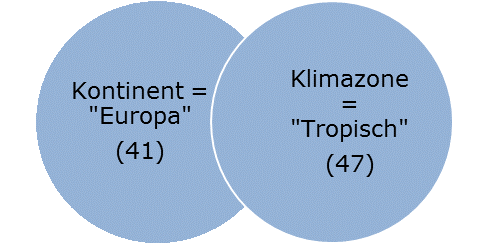
\includegraphics[width=0.5\textwidth]{grafiken/Filter_Vereinigung.png}
 \caption{Vereinigungsmenge Filter}
 \label{fig:filter1}
\end{figure}

Den Wert „Europa“ unter dem Attribut „Kontinent“ haben 41 Länder gesetzt, den Wert „Tropische Klimazone“ unter dem Attribut „Klimazone“, 47 Länder. Die Ergebnismenge besteht nun aus allen Objekten, die mindestens eine der beiden Bedingungen erfüllen, also den 47 Objekten der Klimazonenbedingung und den 41 Ländern, die in Europa liegen. Natürlich werden die Werte, die beiden Bedingungen entsprechen nur einmal in der Ergebnismenge auftauchen (äquivalent zur Vereinigungsmenge). In diesem Beispiel käme man auf 84 Länder, die den Filtereinstellungen entsprechen.

\textbf{Problematik und Konzept}

Der Filter soll für die Anwendungsfälle 2 und 3 angepasst werden. Der Wunsch des Kunden ist eine Mischung aus dem additiven Filter, der bereits existiert, und einem Filter, bei dem die Filterauswahl die Ergebnismenge wieder einschränkt.

Die Ergebnismenge wird erweitert, wenn Werte des gleichen Attributes ausgewählt werden. Die Einschränkung hingegen geschieht, wenn Werte eines anderen Attributes ausgewählt werden.

Auch hier hilft die Mengenlehre, das Verhalten des Filters zu verdeutlichen (Anwendungsfall 2):

Schritt 1 – Auswahl aus Attribut Motor:
\begin{itemize}
	\item Motor A
	\item Motor B
\end{itemize}

\begin{figure}[H]
 \centering
 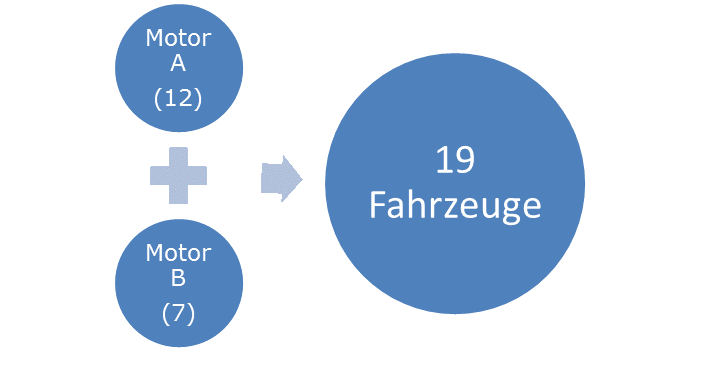
\includegraphics[width=0.7\textwidth]{grafiken/Filter_Motor.png}
 \caption{Teilmenge 1 - Exklusivfilter}
 \label{fig:filter2}
\end{figure}

Zu diesem Zeitpunkt besteht die Ergebnismenge aus genau diesen Fahrzeugen. Die Anzahl an Fahrzeugen der beiden Werte „Motor A“ und „Motor B“ können ohne weitere Bedenken addiert werden, da es keine Fahrzeuge mit 2 Motoren gibt.

Schritt 2 – Auswahl aus Attribut Getriebe
\begin{itemize}
	\item Getriebe A
	\item Getriebe B
\end{itemize}

\begin{figure}[H]
 \centering
 \includegraphics[width=0.7\textwidth]{grafiken/Filter_Getriebe.png}
 \caption{Teilmenge 2 - Exklusivfilter}
 \label{fig:filter3}
\end{figure}

Bei der Auswahl in Schritt 2 würden 15 Fahrzeuge in der Ergebnismenge landen. Da jetzt aber über zwei verschiedene Attribute gefiltert wird, muss die Ergebnismenge aus den beiden einzelnen Ergebnissen berechnet werden. Dazu bilden wir die Schnittmenge der beiden Teilmengen.

\begin{figure}[H]
 \centering
 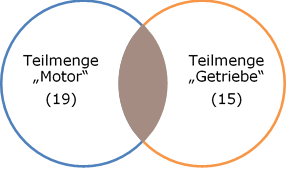
\includegraphics[width=0.5\textwidth]{grafiken/Filter_Schnitt.png}
 \caption{Schnittmenge - Exklusivfilter}
 \label{fig:filter4}
\end{figure}

Die Ergebnismenge ist in der Grafik genau der Bereich, in dem sich die beiden Teilmengen überschneiden. Sie enthält alle Elemente, die sowohl in der einen als auch in der anderen Teilmenge vorkommen.

Bei der Übernahme des Konzeptes auf die tatsächliche Implementierung des Filters, muss allerdings bedacht werden, dass die Schnittmenge aus einer Vielzahl an Attributen berechnet werden muss.

Zur Verbesserung der Gebrauchstauglichkeit des Filters müssen in diesem Fall nach Selektion von Werten eines Attributes die Wertelisten der anderen Attribute aktualisiert werden, sodass durch die alleinige Auswahl von Werten verschiedener Attribute kein leeres Ergebnis entstehen kann.

Im Umkehrschluss bedeutet das Vorhergegangene allerdings, dass die Wertelisten auch jedes Mal aktualisiert werden müssen, wenn ein Wert wieder aus der Filterselektion „rausgeworfen“ wird. Dies muss auch geschehen, wenn sich dadurch eine gerade betrachtete Werteliste ändert.

\textbf{Umsetzung}

Auf technischer Seite ist der Filter so implementiert, dass es definierte Datenstrukturen für alle relevanten Mengen gibt. Folgende Strukturen existieren:

\begin{itemize}
	\item Menge aller Filterattribute
	\item Alle Wertelisten, zugeordnet zu einem Filterattribut
	\item Zuordnung von Wertelisten mit (noch) selektierbaren Werten zu jeweils einem Attribut
	\item Menge aller Filterattribute, von denen mindestens ein Wert selektiert wurde
	\item Zuordnung selektierter Werte zu einem Filterattribut aus zuvor genannter Menge
\end{itemize}

Um die obigen Mengen aktuell zu halten, also Änderungen in allen Mengen quasi-gleichzeitig zu publizieren werden JavaFX-Listener benutzt. Wird die Menge der selektierten Werte geändert, werden die anderen Mengen aktualisiert.

Der Filter wird durch einen DataProvider und durch einen FilterDataProvider gestützt. Der DataProvider liefert alle existierenden Modellobjekte, die behandelt werden sollen und der FilterDataProvider stellt die Attribute sowie die verfügbaren Werte zur Verfügung.

Die Logik führt bisher die in dem Abschnitt Ausgangssituation beschriebenen Mengenoperation mit einigen Besonderheiten aus. So gibt es zum Beispiel unterschiedliche Attributtypen. Es gibt ValueListFilterAttributes, die die oben genannten Wertelisten beinhalten, BooleanFilterAttributes, die nur die Werte Ja und Nein beinhalten und es gibt ParentFilterAttributes, die dazu dienen, andere FilterAttribute zu gruppieren und diese Filterattribute als Sublisten der ParentFilterAttribute darzustellen. Um die Beschreibung der Änderungen auf das Wesentliche zu reduzieren, wird auf diese und weitere Eigenheiten nicht näher eingegangen.

Die Änderungen am Quellcode umfassen im Groben folgendes:

Für die Methode \#isInFilter(Modelobjekt), die überprüft, ob ein Objekt den gewählten Filterkriterien entspricht, wurde eine Fallunterscheidung eingeführt. Diese erlaubt es, dass der Filter für den Anwendungsfall 1 wie bisher funktioniert, für den 2. Anwendungsfall jedoch das Schnittmengenkonzept implementiert. Dazu wird für jedes selektierte Attribut überprüft, ob der Wert, den das Modelobjekt für das entsprechende Attribut gesetzt hat, in der Menge der selektierten Werte vorhanden ist. Ist dies für ein Attribut nicht der Fall, bedeutet das, das geprüfte Modelobjekt darf nicht in der Ergebnismenge vorhanden sein.

Auch die Wertelisten mit den auswählbaren Werten aktualisieren sich jetzt zeitgleich mit der Filterselektion. Dies erforderte mehr Aufwand, da die Wertelisten nach Definition nur durch die Selektion von Werten eingeschränkt werden dürfen, die einem anderen Attribut zugeordnet sind als die betrachtete Werteliste. Um dies zu realisieren wurde eine neue Menge zu den oben beschriebenen Mengen hinzugefügt, die parallel zu den selektierbaren Werten eine gefilterte Sicht auf diese Werte bietet. Um die einzelnen Listen zu erzeugen, die jeweils einem Attribut zugeordnet sind, benötigt es zum einen eine Änderung an der \#isInFilter(Modelobjekt) Methode und zum Anderen die Aktualisierung bei Änderung der selektierten Werte. Bei der \#isInFilter(Modelobjekt) Methode kam ein neuer Parameter hinzu, welcher ein zu ignorierendes Attribut entgegennimmt. Das „Exklusiv-Attribut“ wird dann bei der darauf folgenden Berechnung nicht mit einbezogen.

\begin{lstlisting}[
    language=Java,
    caption=Auszug aus Code der Methode \#isInFilter(Modelobjekt\, Filterattribut),
    label=code9]
	[...]
	for (AbstractFilterAttribute<A> attribute : selectedAttributes) {
		if (!attribute.equals(exclusiveAttribute)) {
			Object attributeValue = dataProvider.resolve(dataObject, attribute.getAttributeName());
			if (!isValueSelected(attribute, value)) {
					return false;
			}
    	}
	}
	return !selectedValues.isEmpty();
	// returns true when loop passed through and false when there is no selection
	[...]
\end{lstlisting}

Diese Berechnung wird für jedes Modelobjekt ausgeführt um festzustellen, ob es in der Ergebnismenge inbegriffen ist, oder nicht. Die einzelnen, den Attributen zugeordneten, Wertelisten der nicht-selektierten Werte, begründen sich gemäß der Implementierung auf der Berechnung einer Pseudo-Ergebnismenge, die das Attribut der betrachteten Werteliste nicht berücksichtigt. Die Attributwerte aller übrig gebliebenen Modelobjekte, die nicht in der Pseudo-Ergebnismenge vorhanden sind, dienen dazu, die spezielle Werteliste zu befüllen. So wird vermieden, dass Filterwerte angewählt werden, die zu einer leeren Ergebnismenge führten.

Andersherum betrachtet ist es nicht so einfach möglich, zu verhindern, dass durch das „rauswerfen“ von Attributwerten aus der Filterselektion, eine leere Ergebnismenge geschaffen wird. Um dies zu realisieren, müsste die Handlungsfreiheit des Nutzers stark eingeschränkt werden und verhindert werden, dass solche Attributwerte deselektiert werden. Zudem erforderte dies eine ständige Neuberechnung der möglichen Ergebnismenge, falls ein bestimmter Wert aus der Filterauswahl „geworfen“ werden würde – und dies für jeden möglichen Wert, der entfernt werden kann.

\section{DataProvider} \label{sec:implDataProvider}
\textbf{Struktur}

Der DataProvider versorgt, wie der Name schon andeutet, die einzelnen Bereiche der Anwendungslogik mit Daten aus dem Model. Es gibt für jeden Anwendungsfall einen eigenen DataProvider, da jedes Szenario auf einer eigenen Art von Modelobjekten beruht. Die Klasse stellt neben den Modellobjekten weitere Methoden zum Auflösen von Attributwerten bereit. Dazu nimmt die Methode ein Modellobjekt und ein Attribut entgegen und liefert den dazugehörigen Wert zurück.

\begin{figure}[H]
 \centering
 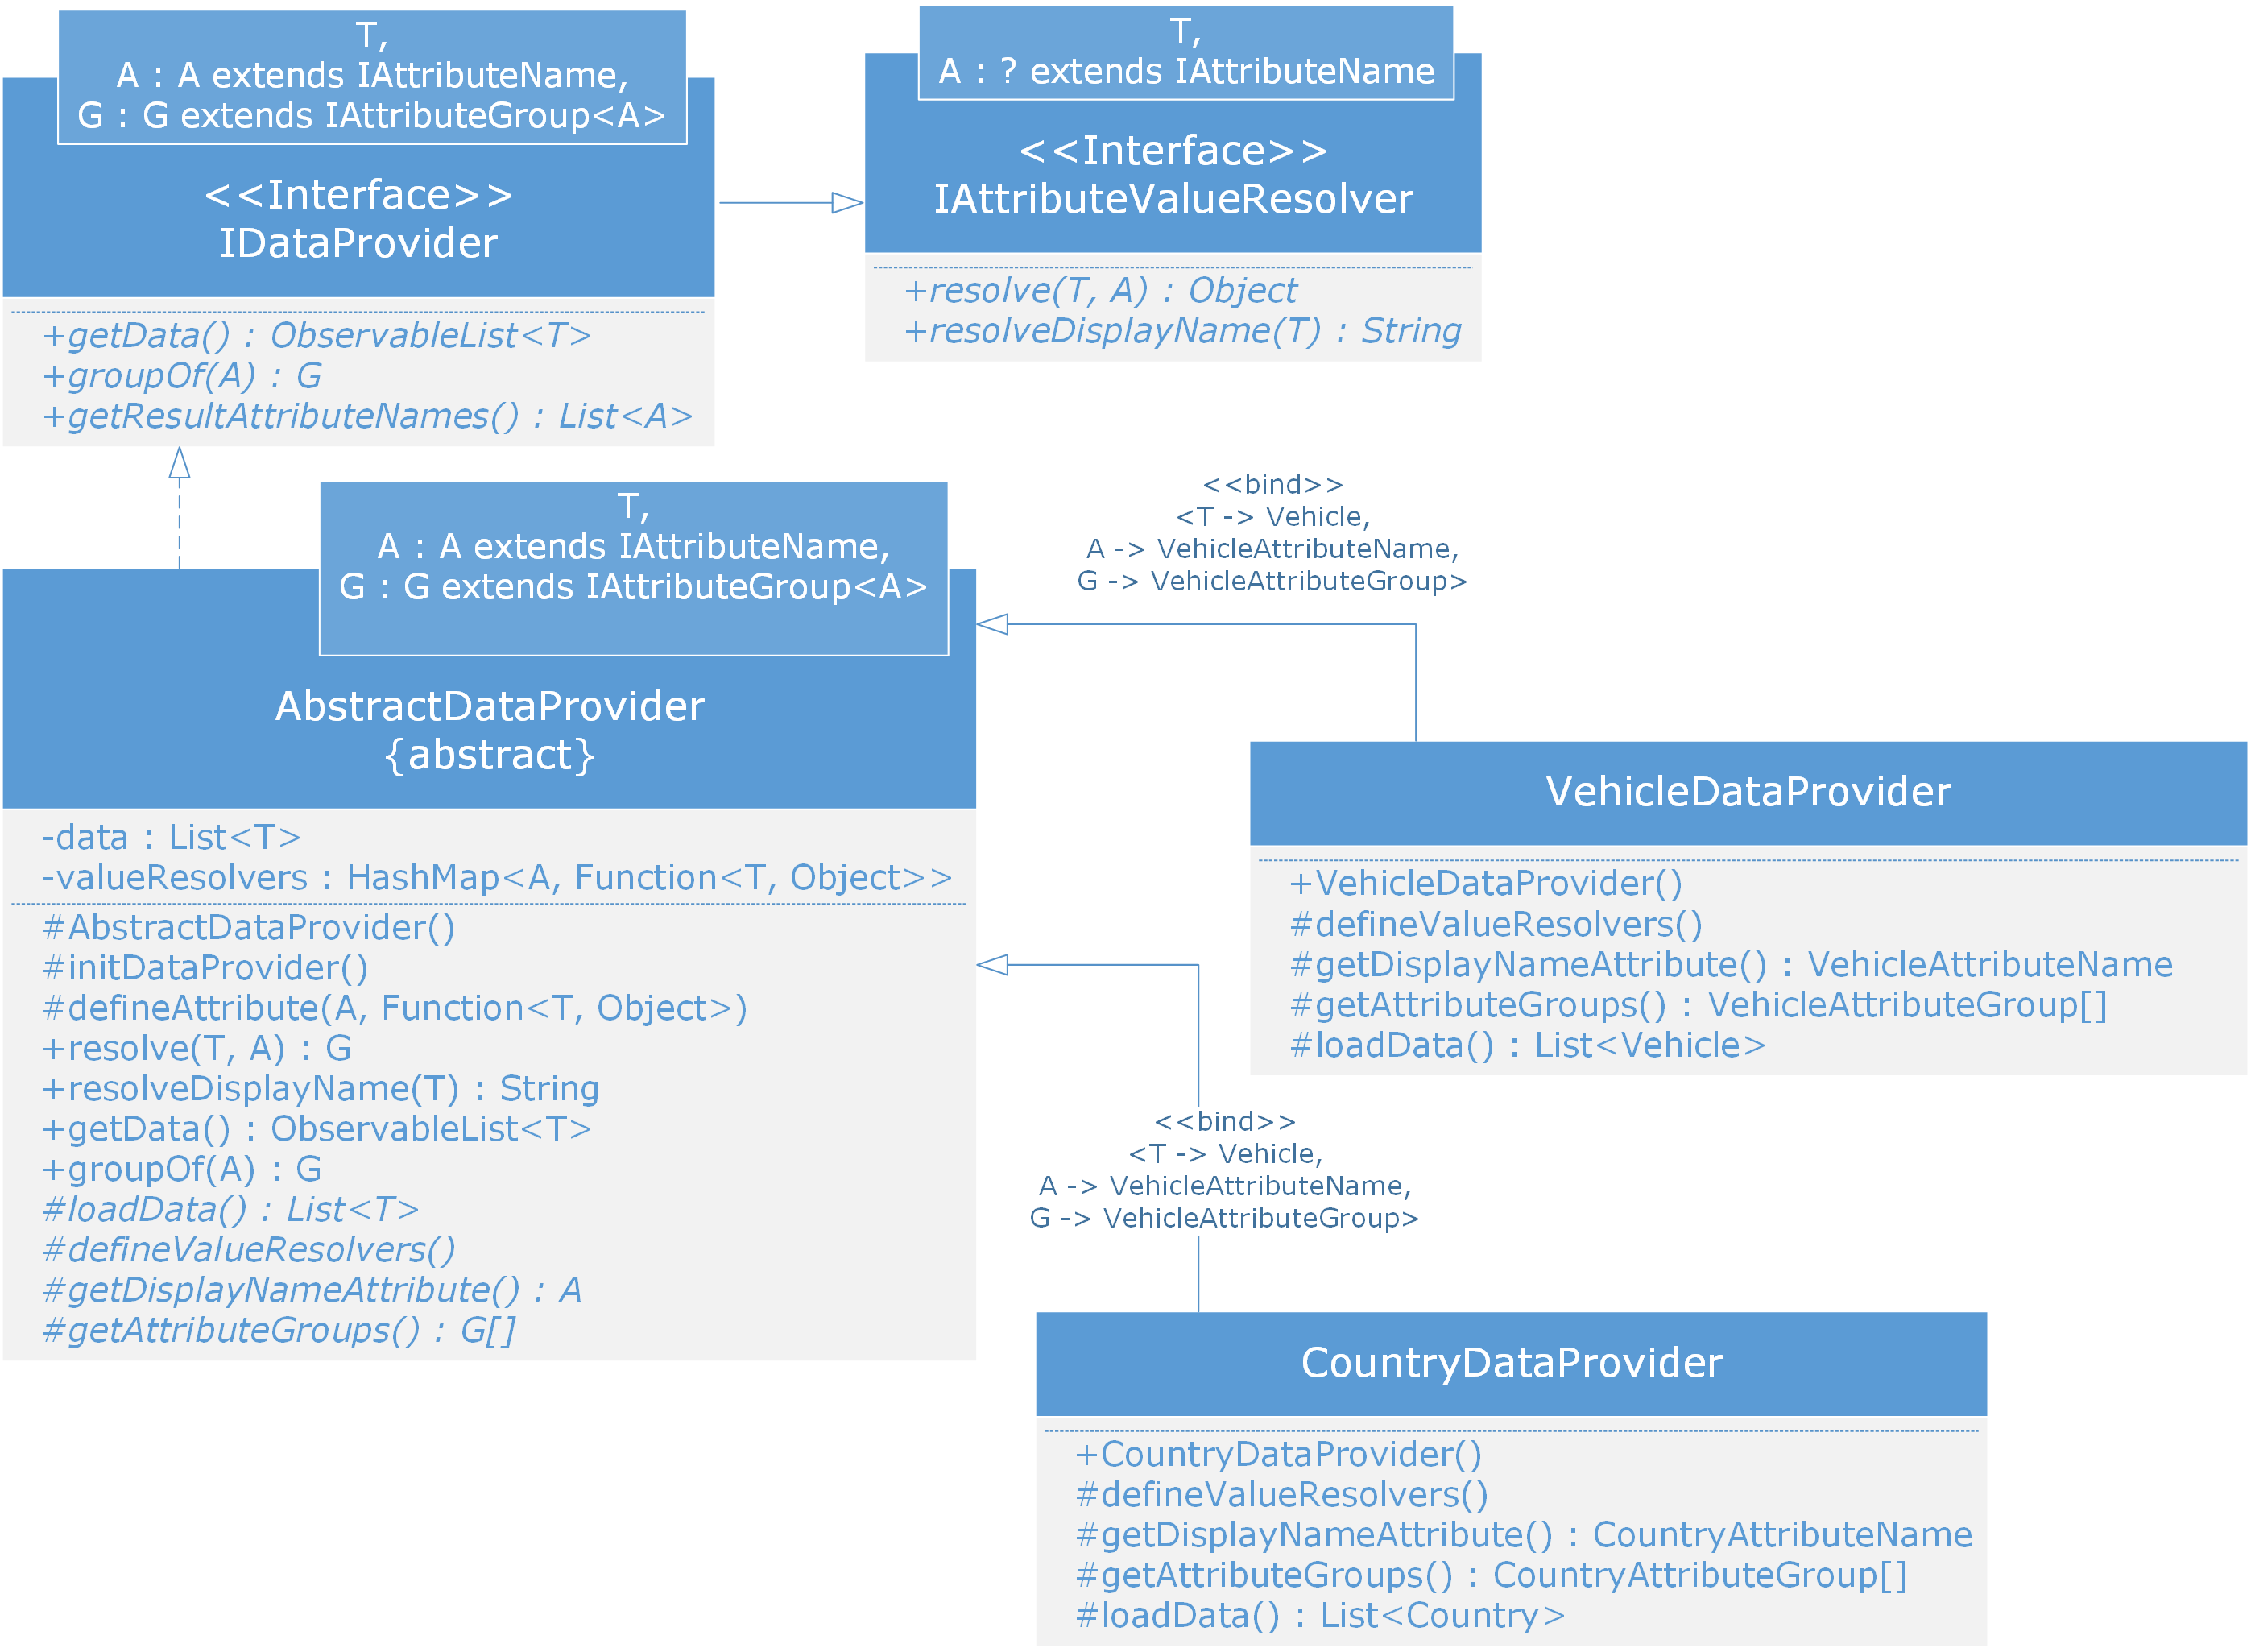
\includegraphics[width=1\textwidth]{grafiken/Class_DataProvider.png}
 \caption{Klassendiagramm DataProvider}
 \label{fig:dataProvider1}
\end{figure}

Die bestehende Klassenstruktur enthält bereits Interfaces und abstrakte Klassen, welche die Implementierungsstruktur eines DataProviders vorgeben. Die Grafik zeigt einen Ausschnitt der Klassenhierarchie und stellt die zum Verständnis relevanten Member dieser Klassen dar. Das hierarchisch höchste Interface IAttributeValueResolver liefert Funktionen, die für das Auflösen spezieller Werte zuständig sind. Anhand eines Modelobjektes T, mit dem das Interface als generischer Parameter wurde, und einem Attribut, das das Interface IAttributeName implementieren muss, kann ein Wert erhalten werden (z.B. „Spanien“ für das Attribut Land).
Ein weiteres Interface stellt der IDataProvider dar, der von IAttributeValueResolver ableitet. Hier werden Methoden definiert, um die Modelobjekte dieses DataProviders zu erhalten. Außerdem kann man per Methodenaufruf die Attribute bekommen, die für die Ergebnisanzeige benötigt werden und die Zuordnung eines Attributes zu einer Attributgruppe.

Der AbstractDataProvider bietet nun die ersten Implementierungen für die abstrakten Methoden der Interfaces an. Zusätzlich werden weitere abstrakte Methoden hinzugefügt, die die konkrete Implementierung durch Unterklassen erfordern. Die Methoden werden für das Laden der Daten aus der Datenbank, sowie der Definition von ValueResolvers  benötigt. Ein ValueResolver beschreibt mithilfe einer Java8-Function, wie für ein bestimmtes Attribut bei Eingabe eines Modelobjektes T, der Wert für dieses Attribut erhalten werden kann. Ein Resolver ist immer einem Attribut zugeordnet.

\textbf{Problemstellung}

Es soll parallel zu dem CountryDataProvider und dem VehicleDataProvider der DataProvider für den 3. Anwendungsfall implementiert werden. Dazu gehört die Definition der Attribute, die durch das Interface IAttributeValueResolver benötigt werden, mit der jeweiligen Zuordnung zu einer Attributgruppe. Zusätzlich muss eine Datenstruktur entwickelt werden, die die geladenen Informationen in einem Objekt zusammenfasst – also die kombinierten Länder und Fahrzeugdaten zusammen mit den Produktionsfreigaben.

\textbf{Umsetzung}

Zunächst müssen die Attribute definiert werden. Diese sind abhängig von der Ergebnispräsentation. Per Anforderung sollen in der Ergebnistabelle Details zu den Fahrzeugen angezeigt werden und die Start/ Enddaten der Produktionsfreigaben. Daher entsprechen die definierten Attribute in erster Linie den Attributen aus dem Fahrzeug-Szenario. Aus diesem Grund müssen die Attribute nicht alle neu definiert werden, sondern können durch eine statische Methode \#createAttributeName(IAttributeName) erzeugt werden. Das neu erzeugte Attribut dient nur als Kapselung für das eigentliche Attribut, welches aus der Menge der Fahrzeug-Attribute kommt. Die Methode wird für jedes Fahrzeug-Attribut durch die bei der Definition der Attributgruppen aufgerufen. In dem Enum der Attributgruppen werden dem Konstruktor die Original-Attributgruppen übergeben und die Attribute für den 3. Anwendungsfall können per Iteration über die zugeordneten Attributnamen erzeugt werden. Um zu vermeiden, dass Attribute mehrfach definiert werden, werden die gekapselten Attribute in einer statischen Map gespeichert, die als Key das Original-Attribut enthält und als Value den Wrapper zur Verfügung stellt. Zusätzlich zu den Wrapper-Attributen gibt es statische Attribute, die für die Produktionsfreigabedaten stehen.

Im DataProvider müssen, nachdem die Attribute erzeugt wurden, die ValueResolvers beschrieben werden. Es muss also für jeden Attributnamen eine Function implementiert werden. Allerdings kann, durch überschreiben der \#resolve(Modelobjekt, AttributeName)-Methode doppelter Code vermieden werden. Wie bereits erläutert, stammen viele der Attribute aus dem Fahrzeug-Anwendungsfall und so kann der Original-DataProvider genutzt werden, um die Werte für die meisten Attribute aufzulösen. Es müssen nur noch die Resolver für die hinzugekommenen Attribute definiert werden.

In der Theorie werden für den 3. Anwendungsfall die Daten aus dem Länder-Anwendungsfall mit den Daten aus dem Fahrzeug-Anwendungsfall kombiniert und mit zusätzlichen Daten, den Produktionsfreigaben versehen. Dies geschieht für jede Kombination aus Fahrzeugen und Ländern, für die es eine Produktionsfreigabe gibt. Da die Menge an Produktionsfreigaben mit allen daran registrierten Daten lange Ladezeiten und sehr viel Speicher erfordern würde, können die Produktionsfreigaben vorab nicht geladen werden. Stattdessen werden, um Werte für den Filter bereitzustellen, zunächst nur die Länder- und die Fahrzeugdaten aus der Datenbank geladen. Gekapselt werden diese Daten in einer Datenstruktur FilterElement. Diese Struktur wird im nächsten Kapitel genauer erläutert.

\section{Multi-Filter} \label{sec:implMulti-Filter}
\textbf{Problemstellung}

Für den neuen Anwendungsfall ändern sich nun auch die Anforderungen an den Filter. Die Auswahl beruhte bislang nur auf Modellobjekten, die fachlich genau eine Art von anzuzeigenden Daten repräsentierten. Die Länderobjekte stellten Länder mit gewissen Eigenschaften dar und die Fahrzeugobjekte standen für Fahrzeuge. Die Modellobjekte für die neuen Funktionen hingegen bestehen nach dem Laden der Daten aus 2 verschiedenen Datensätzen (Land und Fahrzeug) und zur Zeit der Anzeige sogar aus 3 Datensätzen (zusätzlich die Produktionsfreigabe-Objekte).

Die Ergebnismenge, die auf dem Filter basiert, soll frei konfigurierbar sein. Das bedeutet, es sollen Produktionsfreigaben für eine beliebige Kombination von Ländern mit Fahrzeugen angezeigt werden können. Um das zu ermöglichen werden zwei voneinander unabhängig konfigurierbare Filter benötigt, die im Endeffekt jedoch zu einer einzelnen Ergebnismenge führen. Die einzelnen Filter sollen analog zu ihren jeweiligen ursprünglichen Anwendungsfällen implementiert werden. Der Länderfilter soll additiv funktionieren (siehe Kap. ?) und der Fahrzeug-Filter einschränkend (sieh Kap. ?).

Nach der Auswahl der Filterwerte müssen die Produktionsfreigaben in die Land-Fahrzeug-Kombinationen eingefügt werden.

\textbf{Umsetzung}

Die erste Problematik bezieht sich darauf, wie ein solcher Filter umzusetzen ist. Eine Möglichkeit wäre es, die Klasse Filter dahingehend umzuschreiben, dass sie sowohl mit einem als auch mit 2 Modellobjekten arbeiten kann. Der Vorteil dieser Lösung läge vor Allem darin, dass nur wenige Klassen bearbeitet werden müssten.
Eine andere Möglichkeit ist, die Filterlogik zu belassen und stattdessen die umgebende Struktur so zu verändern, dass 2 Instanzen des Filters gleichzeitig und unabhängig voneinander verwendet werden können.

Da die Logik der Filter-Klasse mit verschiedenen Sonderbehandlungen ohnehin schon recht komplex ist, ist die zweite Möglichkeit in diesem Falle zu bevorzugen.
Folgend ist die Methodenschnittstelle der Filter-Klasse aufgeführt.

\begin{figure}[H]
 \centering
 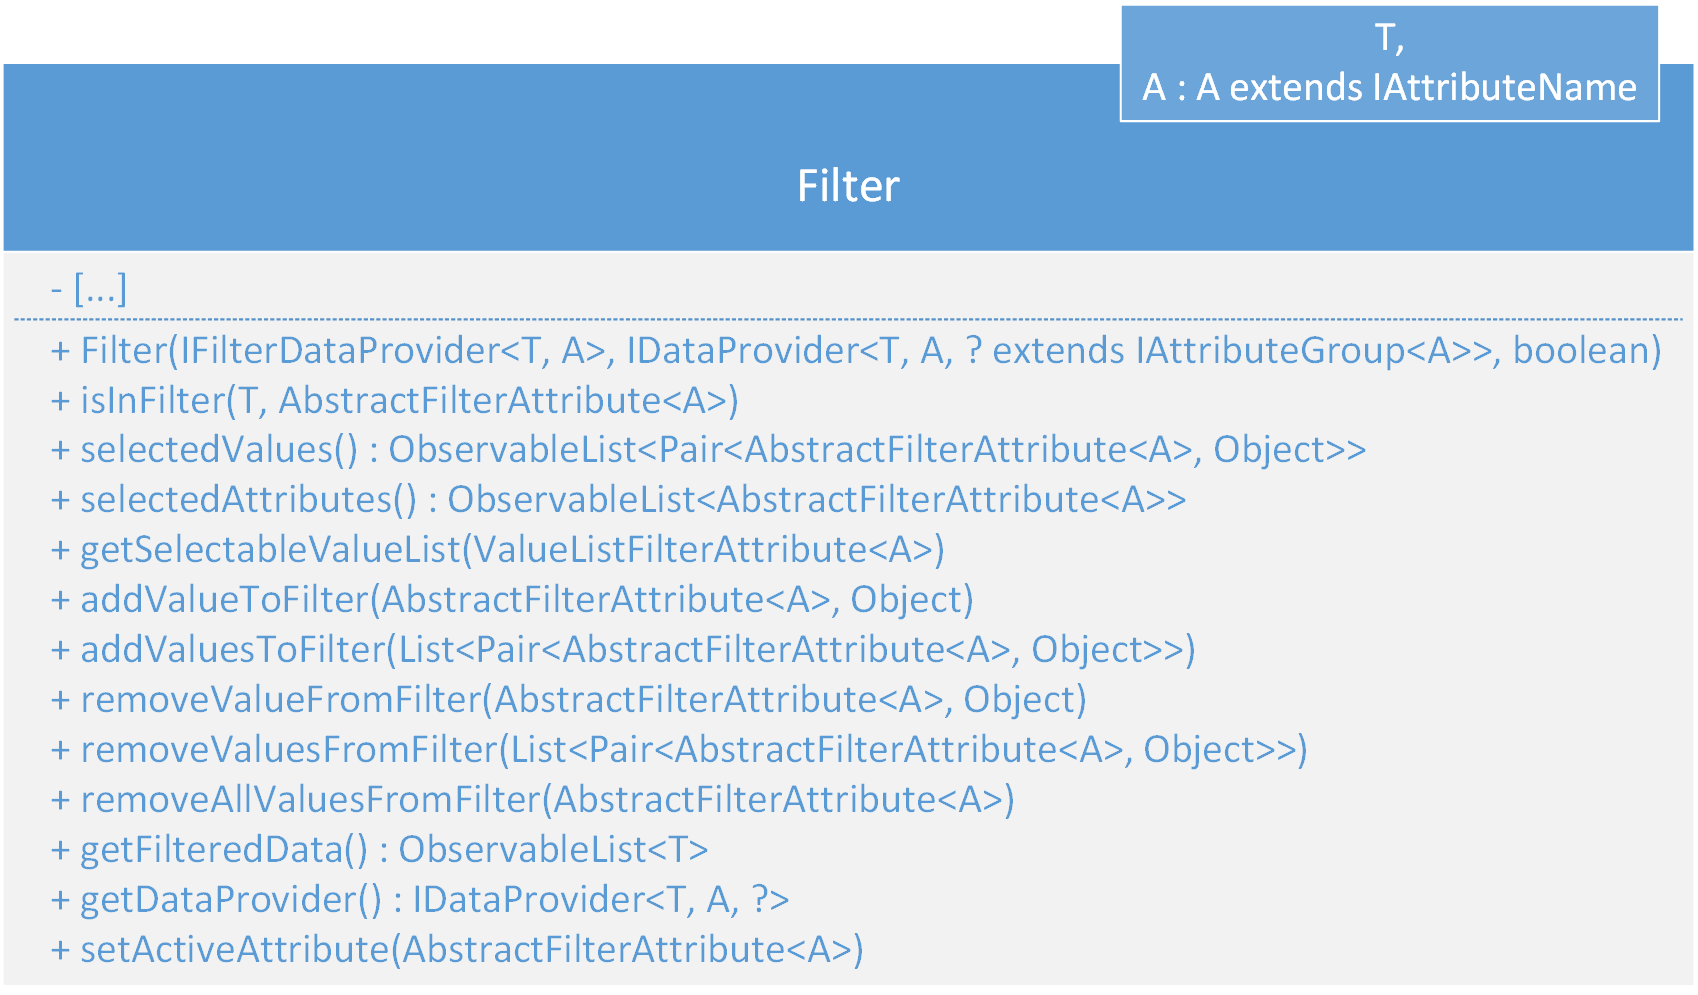
\includegraphics[width=0.85\textwidth]{grafiken/Class_Filter.png}
 \caption{Klassenaufbau - Filter}
 \label{fig:multiFilter1}
\end{figure}

Die Schnittstelle bietet Methoden, um auf die in "Kapitel 3.1 – Umsetzung" definierten Mengen zuzugreifen. Es zeigt sich, dass einige Mengen  nicht ganz wie erwartet implementiert sind. Im Beispiel der selectedValues wird eine ObservableList (JavaFX) vom Typ Pair<AbstractFilterAttribute<A>, Object> verwendet, anstatt der naheliegenden Map mit der Typisierung <AbstractFilterAttribute<A>, List<Object>>. Diese Entscheidung wurde getroffen, da sonst eine Benachrichtigung per JavaFX-Listener über eine Änderung an dieser Menge nur auf umständlichem Wege möglich wäre. Dies ist bei mehreren dieser Mengen der Fall.

Eine weitere Auffälligkeit ist die häufige Verwendung von Generics. Wie bereits zuvor erwähnt, verarbeitet der Filter verschiedene Arten von Modellobjekten. Um dies zu bewerkstelligen, benötigt er nur die Informationen aus dem bereits erläuterten DataProvider und weitere Information aus einem FilterDataProvider. Neben dem Filter gibt es noch viele weitere Klassen, die generisch implementiert sind.

Für den FilterDataProvider gibt es ebenfalls pro Anwendungsfall eine spezifische Implementierung. Für die Aufgabe ist dieser Teil der Logik jedoch nur bedingt relevant. Im Wesentlichen erstellt der FilterDataProvider aus den Modellobjekten des spezifischen Szenarios die Wertelisten für jedes Attribut zusammen indem er alle Modellobjekte durchläuft, die verschiedenen Werte zusammenträgt und gleiche Elemente zu einem zusammenfasst.

Um die Filteranforderungen umzusetzen muss nun eine Klasse geschrieben werden, die 2 dieser Filter verwaltet und Methodenaufrufe entsprechend delegiert. Dies kann wieder auf verschiedene Arten geschehen. Eine Möglichkeit wäre es, eine Art Provider für den Filter zu entwerfen. An diesem müssten dann Verwendungsstellen den Filter abfragen und würden, je nach Status der Anwendung, den Länder- oder den Fahrzeugfilter zurückbekommen. Da viele Verwendungsstellen den Filter jedoch zwischenspeichern und mit dem Umbau auf eine Providerstruktur auch gleichzeitig die Verwendung eines einzelnen Filters (Anwendungsfall 1 und 2) komplizierter werden würde, ist diese Lösung eher ungeeignet.

Als Alternative dazu kann man einen neuen Filter entwerfen, der die anderen beiden Filter verwaltet. Für die Realisierung muss als Erstes der bestehende Filter abstrahiert werden. Sämtliche Methoden der Schnittstelle des Filters müssen in die Oberklasse verschoben werden. Für diesen Fall bietet es sich an eine Abstrakte Klasse zu konstruieren, von der der bestehende Filter ableitet und die public Methoden der Schnittstelle überschreibt. Diese neue Klasse wird AbstractFilter genannt und bekommt dieselben generischen Typen zugewiesen wie die Klasse Filter. In den Verwendungsstellen muss nur (außer bei dem Konstruktoraufruf) "Filter" durch "AbstractFilter" ersetzt werden und das Programm funktioniert genauso wie zuvor. Für die neue Funktionalität wird eine weitere Klasse eingeführt, die ebenfalls von dem AbstractFilter ableitet und zwei konkrete Instanzen der Filter-Klasse (Länder- und Fahrzeugfilter) verwaltet.

\begin{figure}[H]
 \centering
 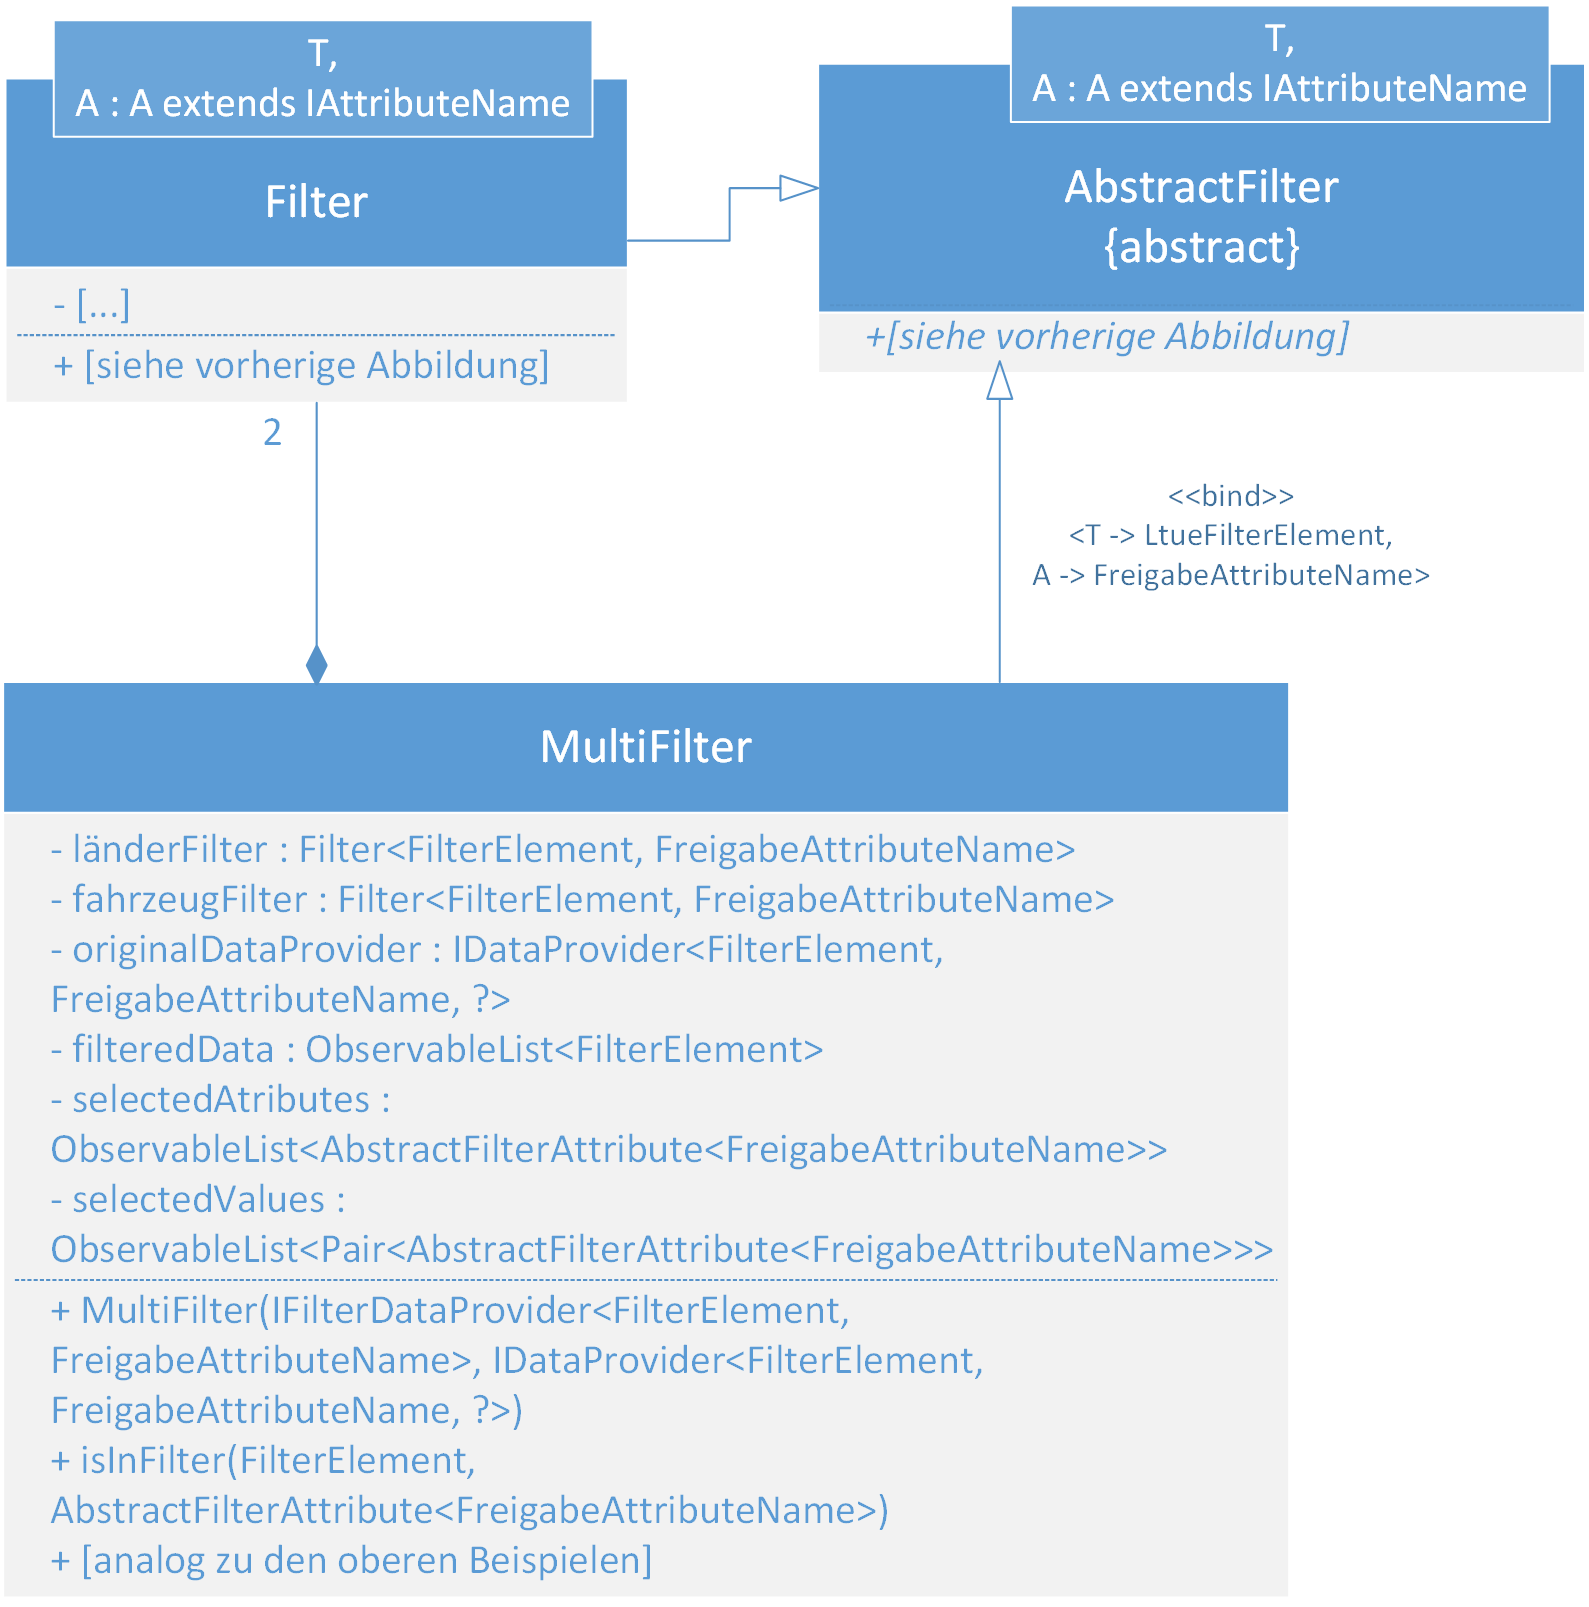
\includegraphics[width=0.85\textwidth]{grafiken/Class_MultiFilter.png}
 \caption{Klassendiagramm - Konzept Filter}
 \label{fig:multiFilter2}
\end{figure}

In der Abbildung 3.7 sind die neuen Beziehungen zwischen den Filter-Klassen visualisiert. Um diese Struktur verwenden zu können, muss im 3. Anwendungsfall, statt eines normalen Filters, der neue MultiFilter initialisiert werden. Wie dem Entwurf der MulitFilter-Klasse (Abb. 3.7) entnommen werden kann, erwartet der MultiFilter als Modelobjekte die FilterElemente. Diese sind dreiteilig aufgebaut.

\begin{enumerate}
	\item Der Länderteil
	\item Der Fahrzeugteil
	\item Der Freigabeteil
\end{enumerate}

Mit Gettern und Settern kann auf diese zugegriffen werden. Die Problematik besteht an dieser Stelle zunächst darin, ein FilterElement einem der zwei Sub-Filter zuzuordnen. Dies wird realisiert, indem die FilterElemente, die in einer einzelnen Liste vom DataProvider zur Verfügung gestellt werden, verschiedene Ausprägungen besitzen. Wie in Kapitel 3.2 beschrieben, werden die Länder- und die Fahrzeugdaten getrennt voneinander geladen. Daher können bereits im DataProvider die FilterElemente verschieden erzeugt werden. Der eine Teil der FilterElemente hat nur die Membervariable für das Land gesetzt, der andere Teil der Objekte nur die Variable für das Fahrzeug. So kann der MultiFilter die Elemente eindeutig einem konkreten Filter zuordnen.

Die beiden einzelnen Filter können daraufhin unabhängig voneinander die Ergebnismenge bestimmen. Diese Mengen werden von dem MultiFilter zu einer Ergebnismenge zusammengeführt. Für diesen Zweck bietet die Klasse FilterElement eine statische Methode \#merge(FilterElement, FilterElement) an, die ein FilterElement zurückliefert, das sowohl die Ländervariable als auch die Fahrzeugvariable gesetzt hat.

\begin{figure}[H]
 \centering
 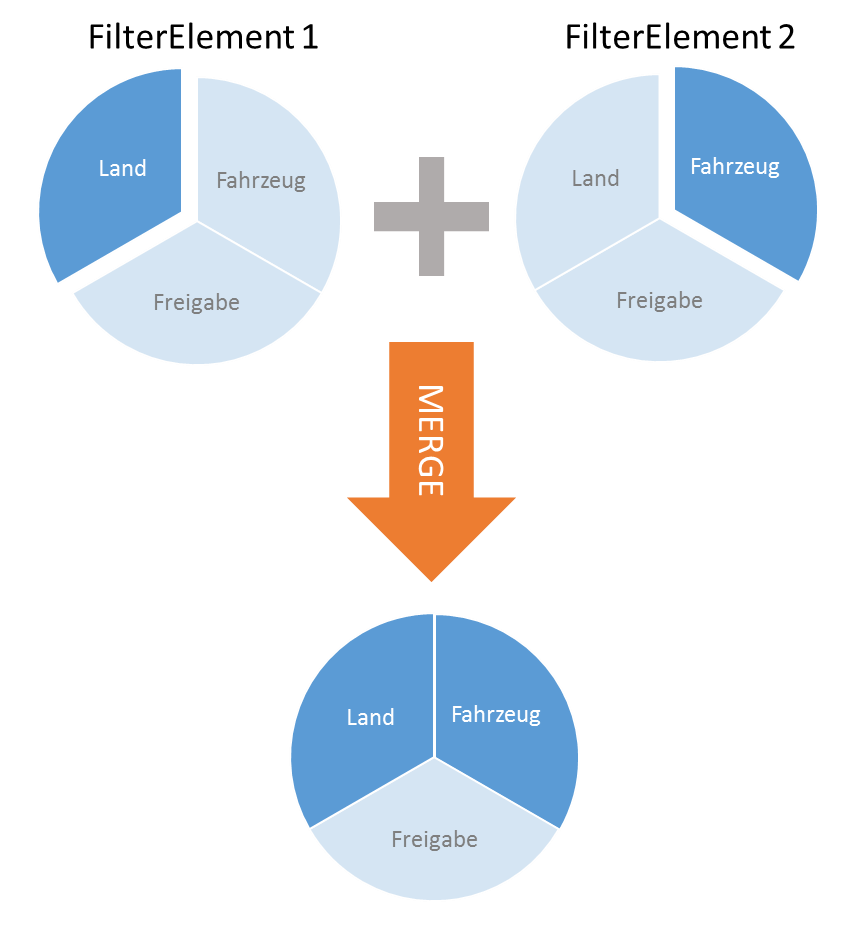
\includegraphics[width=0.65\textwidth]{grafiken/Multi_FilterElement.png}
 \caption{Schema FilterElement-Aufbau}
 \label{fig:multiFilter3}
\end{figure}

Ist der Vereinigungsvorgang nicht erfolgreich, weil zum Beispiel zwei Länder-FilterElemente übergeben wurden, wird eine IllegalArgumentException geworfen.
Dieser Vorgang wird zur Erzeugung der Ergebnismenge für die Ergebnisansicht durchlaufen. Dies geschieht für jede mögliche Kombination der Elemente aus der Länder-Ergebnismenge mit den Elementen der Fahrzeugmenge. Es wird so das Kartesische Produkt (Abb 3.9) der Mengen gebildet.

\begin{figure}[H]
 \centering
 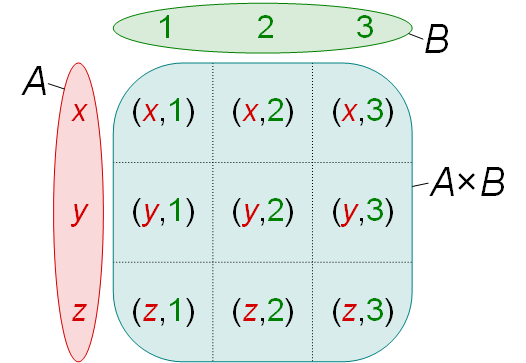
\includegraphics[width=0.4\textwidth]{grafiken/Multi_Kartesisches.png}
 \caption{Kartesisches Produkt}
 \label{fig:multiFilter4}
\end{figure}

Es ist leicht vorstellbar, dass die Elemente der Ergebnismenge und so auch die Anzahl ausgeführter Vereinigungen schnell anwachsen, wenn die Teilmengen größer werden. Die Komplexität dieses Programmteiles ist in der Groß-O-Notation $O(n^2)$. Es gibt aufgrund der Definition des Kartesischen Produktes keinen schnelleren Algorithmus. (Src) Daher muss die \#merge(FilterElement, FilterElement)-Methode möglichst performant implementiert sein und nur ein Minimum an Instruktionen ausführen.

Der letzte Schritt, der für die Erzeugung der endgültigen Ergebnisdaten fehlt, ist das Laden und Setzen der Freigabe-Objekte. Anhand der erzeugten Ergebnismenge kann nun eine Datenbankabfrage durchgeführt werden, die nur eine eingeschränkte Anzahl an Freigabeobjekten lädt. Dazu wird das Command-Pattern benutzt. Es wird also ein Command erzeugt und mit den Fahrzeug- und Länder-IDs an den Server gesendet. Der Server lädt die Freigabedaten daraufhin aus der Datenbank und schickt sie an den Client zurück. Die Ausführung des Commands und das Warten auf die Server-Antwort geschehen in einem anderen Thread als dem GUI-Thread, damit die Benutzeroberfläche nicht \"einfriert". Stattdessen kann während der Ladezeit ein Ladebalken, oder wie im Falle von FalkoFX, eine benutzerdefinierte Ladeanimation angezeigt werden.

\section{Tabellenansicht} \label{sec:implTabelle}
\textbf{Problemstellung}

Die nächste zu bewältigende Anforderung ist die Ergebnispräsentation. Diese soll in einem ersten Schritt als Tabelle erfolgen. An der linken Seite befinden sich als Zeilendeklarator die Fahrzeuge. Für die Spaltenköpfe sind die Länder vorgesehen. Im Inhaltsbereich werden die zu Spalten- und Zeilendeklarator passenden Freigabe-Objekte angezeigt. 

\textbf{Konzept}

Die einzelnen Bildschirme werden bereits über eine zentrale Klasse geladen. Damit ein Bildschirm geladen werden kann, muss eine Klasse das Interface IScreen implementieren. Es stellt die Methoden \#getContent() und \#initialized() zur Verfügung. Die erste Methode dient dem Zugriff auf ein UI-Objekt, das in den JavaFX-Szenegraphen eingehängt wird und den Content-Bereich der Anwendung füllt. Unter diesem JavaFX-Node können weitere Knoten hängen, die den Aufbau einer komplizierten Benutzeroberfläche ermöglichen. Die zweite Methode dient als Callback und wird ausgeführt, sobald die Benutzeroberfläche initialisiert und angezeigt wurde. In dieser Methode können Aktionen ausprogrammiert werden, die erst nach Anzeige des UIs möglich sind (z.B. das Setzen von Daten in eine Tabelle oder das automatische Selektieren einer Zeile).

\begin{figure}[H] 
	\centering
	\subfloat[Schräge Spaltenköpfe] {
		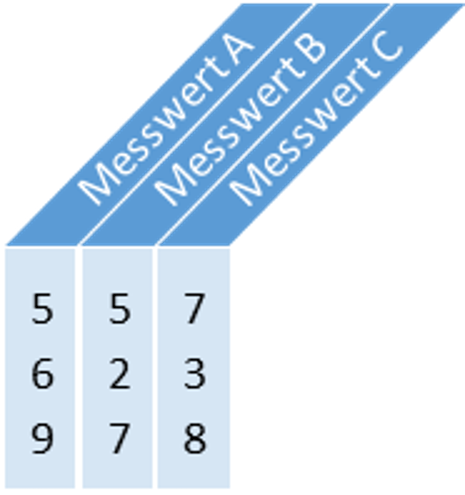
\includegraphics[width=0.25\textwidth]{grafiken/Tabelle_Inclined.png}
	}
	\hspace{2.0em}
	\subfloat[Normale Tabelle] {
		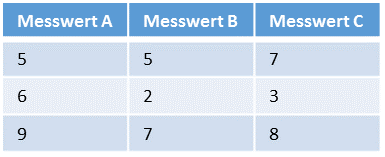
\includegraphics[width=0.5\textwidth]{grafiken/Tabelle_normal.png}
	}
	\caption{Vergleich: Schräge Spaltenköpfe - Normale Tabelle}
	\label{fig:tabelle1}
\end{figure}



Für die Benutzeroberfläche kann eine bereits bestehende Komponente angepasst verwendet werden. Bei der Komponente handelt es sich um eine JavaFX-TableView, die für das FalkoFX-Projekt modifiziert wurde. Eine Besonderheit dieser Tabelle ist, dass sie über schräge Spaltenköpfe verfügt. Dies ist deshalb sinnvoll, damit sich die Spaltenbreite nicht an der Länge des Textes im Spaltenkopf orientieren muss, sondern nur an dem Inhalt der Zellen. Wenn man zuvor weiß, dass es Zellen gibt, die nur sehr kurze Inhalte haben (z.B. ein Icon oder eine kurze Zahl), kann man durch die Verwendung von schrägen Spaltenköpfen den verlorenen Platz minimieren.

Wie man anhand der Abbildungen 3.10 und 3.11 erkennen kann, nimmt zwar die Höhe der Tabelle zu, die Breite wird jedoch viel effektiver ausgenutzt. Der Platz, der am rechten Rand durch die schrägen Spaltenköpfe entsteht, ist bei einer höheren Spaltenanzahl vernachlässigbar gering.

Ein weiterer Vorteil der Tabelle ist die mögliche Gruppierung von Spalten. Diese werden visuell von anderen Gruppen abgetrennt und bilden dementsprechend eine geschlossene Einheit (Abbildung 3.12).

\begin{figure}[H]
 \centering
 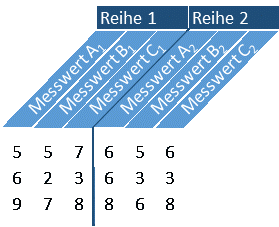
\includegraphics[width=0.5\textwidth]{grafiken/Tabelle_Grouped.png}
 \caption{Schräge Spaltenköpfe mit Gruppierung}
 \label{fig:tabelle2}
\end{figure}

Die Tabelle unterstützt außerdem das ein- und ausblenden von Spaltengruppen, sowie die Umsortierung dieser. In der Anwendung ist diese Funktion in der Seitenleiste untergebracht. (BILD XY?)

Die eigentlichen Informationen, die in der Ergebnisansicht präsentiert werden sollen, sind die Freigabedaten für die Fahrzeugproduktion. Um diese Daten zuordnen zu können, muss Im Spaltenkopf das Land angezeigt werden und am Anfang der Zeile das Fahrzeug mit ausgewählten technischen Daten. Die Informationen zu den technischen Daten sind notwendig, da zu einem Fahrzeug mehrere verschiedene Varianten existieren, die sich in mindestens einem Kriterium unterscheiden. Für jedes dieser Fahrzeuge ist die Freigabe eine andere. 

Wie bereits erwähnt (Kap. 3.2), sind die Hauptinformationen, die man aus einem Freigabe-Objekt erhalten kann, das Start- und das Enddatum der Produktion. Daher ist es sinnvoll, diese beiden Daten auf den ersten Blick anzuzeigen. Dies geschieht, wie auch im Originalclient, durch die Angabe von Kalenderwoche und Jahr nach dem Schema "KW/YY". Daher ist das folgende Layout denkbar:

\begin{figure}[H]
 \centering
 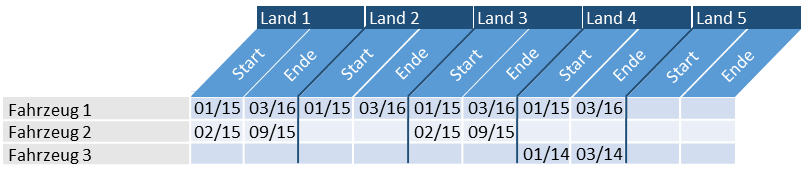
\includegraphics[width=1.0\textwidth]{grafiken/Tabelle_complete.png}
 \caption{Design Ergebnistabelle}
 \label{fig:tabelle3}
\end{figure}

\textbf{Umsetzung}

Die Umsetzung erfordert zunächst die geeignete Benutzeroberfläche. Ein Teil der Implementierungsarbeit ist bereits durch die vorhergegangenen Anwendungsfälle absolviert worden. Auch hier gibt es in beiden Fällen eine Tabellenansicht zur ganzheitlichen Darstellung der Ergebnismenge. Dazu gibt es bislang eine mit Generics parametrisierte Klasse, welche die Ergebnisdarstellung verwaltet. So kann die Darstellung für das erste und das zweite Szenario ohne Änderungen an der Klasse genutzt werden. Auch wenn die Tabelle des dritten Anwendungsfalles denen der anderen beiden vom Aussehen stark ähnelt, kann der bereits existierende Code diese Ansicht nicht erzeugen.

Die bisherige Darstellung ist darauf ausgelegt, dass in jeder Zeile genau ein Modelobjekt mit all seinen Attributwerten angezeigt werden soll. Dabei sind die Spalten mit den entsprechenden Attributnamen betitelt. Die Problematik die hier vorliegt ist jedoch eine andere. Für den Fahrzeugbereich, der in Abbildung 3.13 noch grau angezeigt wird, kann das bisherige Prinzip weiter verwendet werden. Es werden Fahrzeugname und einige weitere technische Details angezeigt, für die wiederum jeweils eigene Spalten mit schrägen Spaltenköpfen existieren (auf Abbildung 3.13 nicht abgebildet). Es ist sinnvoll, dass dieser Bereich an die Ergebniskonfiguration der Seitenleiste gekoppelt ist, da man ggf. mal mehr, mal weniger Details zu den Fahrzeugen einsehen möchte. Für den Hauptbereich allerdings, in dem die Freigabedaten angezeigt werden, funktioniert das bisherige Prinzip nicht. Die Länder, welche die neuen Spaltengruppierungen bilden, sind keine Attribute der dargestellten Modelobjekte, sondern Werte aus der Teilergebnismenge des Filters (Länder-Subfilter), die sich als Teil der Freigabeobjekte wiederfinden.

Nun könnte man eine neue Ergebnisansicht erstellen, die genau dieses Problem behandelt, dann allerdings müsste noch die linke Seite der Tabelle erzeugt werden – die Seite mit den Fahrzeugdaten. Um doppelten Code zu vermeiden, bietet sich hier die Möglichkeit an, die Klasse für die Ergebnisansicht zu abstrahieren und eine generische Klasse für den ersten und zweiten Anwendungsfall davon abzuleiten, sowie eine spezifische Klasse für den 3. Anwendungsfall.

Die JavaFX TableView lässt pro Tabelle nur eine Art von Modellobjekten zu. Diese Objekte stellen dann immer genau eine Zeile dar. Die Werte für die einzelnen Zellen werden mit Hilfe eines CellValueResolvers bestimmt, der pro Tabellenspalte gesetzt wird und so den Wert an einem Schnittpunkt von Tabellenzeile und -spalte bestimmen kann - folglich den Wert einer Zelle. Für die Implementierung bedeutet das, die zusammengesetzten FilterElemente können nicht direkt aus der Ergebnismenge in die Tabelle gesetzt werden, sondern müssen gruppiert und für jede Zeile in einem Objekt zusammengefasst werden. Zu diesem Zweck wird die neue Datenstruktur FreigabeLineObject eingeführt, die eine beliebige Anzahl an Freigabeobjekten enthält, eine Schnittstelle, um auf diese zuzugreifen, sowie eine Möglichkeit das Fahrzeug zu erhalten, nach dem die Werte gruppiert wurden. Aus technischer Sicht wurde die Datenstruktur auf Basis einer HashMap aufgebaut, welche mit Hilfe ID als Key den Zugriff darauf erlaubt. Die Werte der HashMap entsprechen den FilterElementen, welche jeweils ein spezifisches FreigabeObjekt enthalten.

Das Problem, das nun auftritt, ist, dass die Tabellen auf den Modellobjekten (in dem Fall FilterElemente) basieren, es sollen jedoch Elemente vom Typ FreigabeLineObject dargestellt werden. Um dieses Konzept in die vorgestellte Klassenstruktur zu integrieren, muss der AbstractResultTableController mit 2 generischen Parametern versehen werden (Abbildung 3.14). Der erste Parameter steht für den Typ der Modelelemente, auf denen die Ansicht basiert, der zweite Parameter bestimmt den Typen der Zeilenobjekte, die in der Ergebnistabelle landen. Die Unterklassen spezifizieren diese Parameter daraufhin genauer. Es werden außerdem Methoden benötigt, um aus der Ergebnismenge der Modelobjekte die Zielergebnismenge zu generieren und umgekehrt aus einem Zeilenobjekt ein spezifisches Modelobjekt zu erhalten.

Die generische Klasse GenericResultTableController löst das Problem so, dass sie nur noch einen Parameter (T) besitzt, der sowohl für das T als auch das R der Oberklasse steht. Auf diese Weise sind die Modellobjekte gleich den Objekten, die in der Ergebnistabelle pro Zeile angezeigt werden (Abbildung 3.14). Bei dem spezifischen FreigabeResultTableController werden die Parameter mit den konkreten Klassen FilterElement und FreigabeLineObject überschrieben (Abbildung 3.14).

\begin{figure}[H]
 \centering
 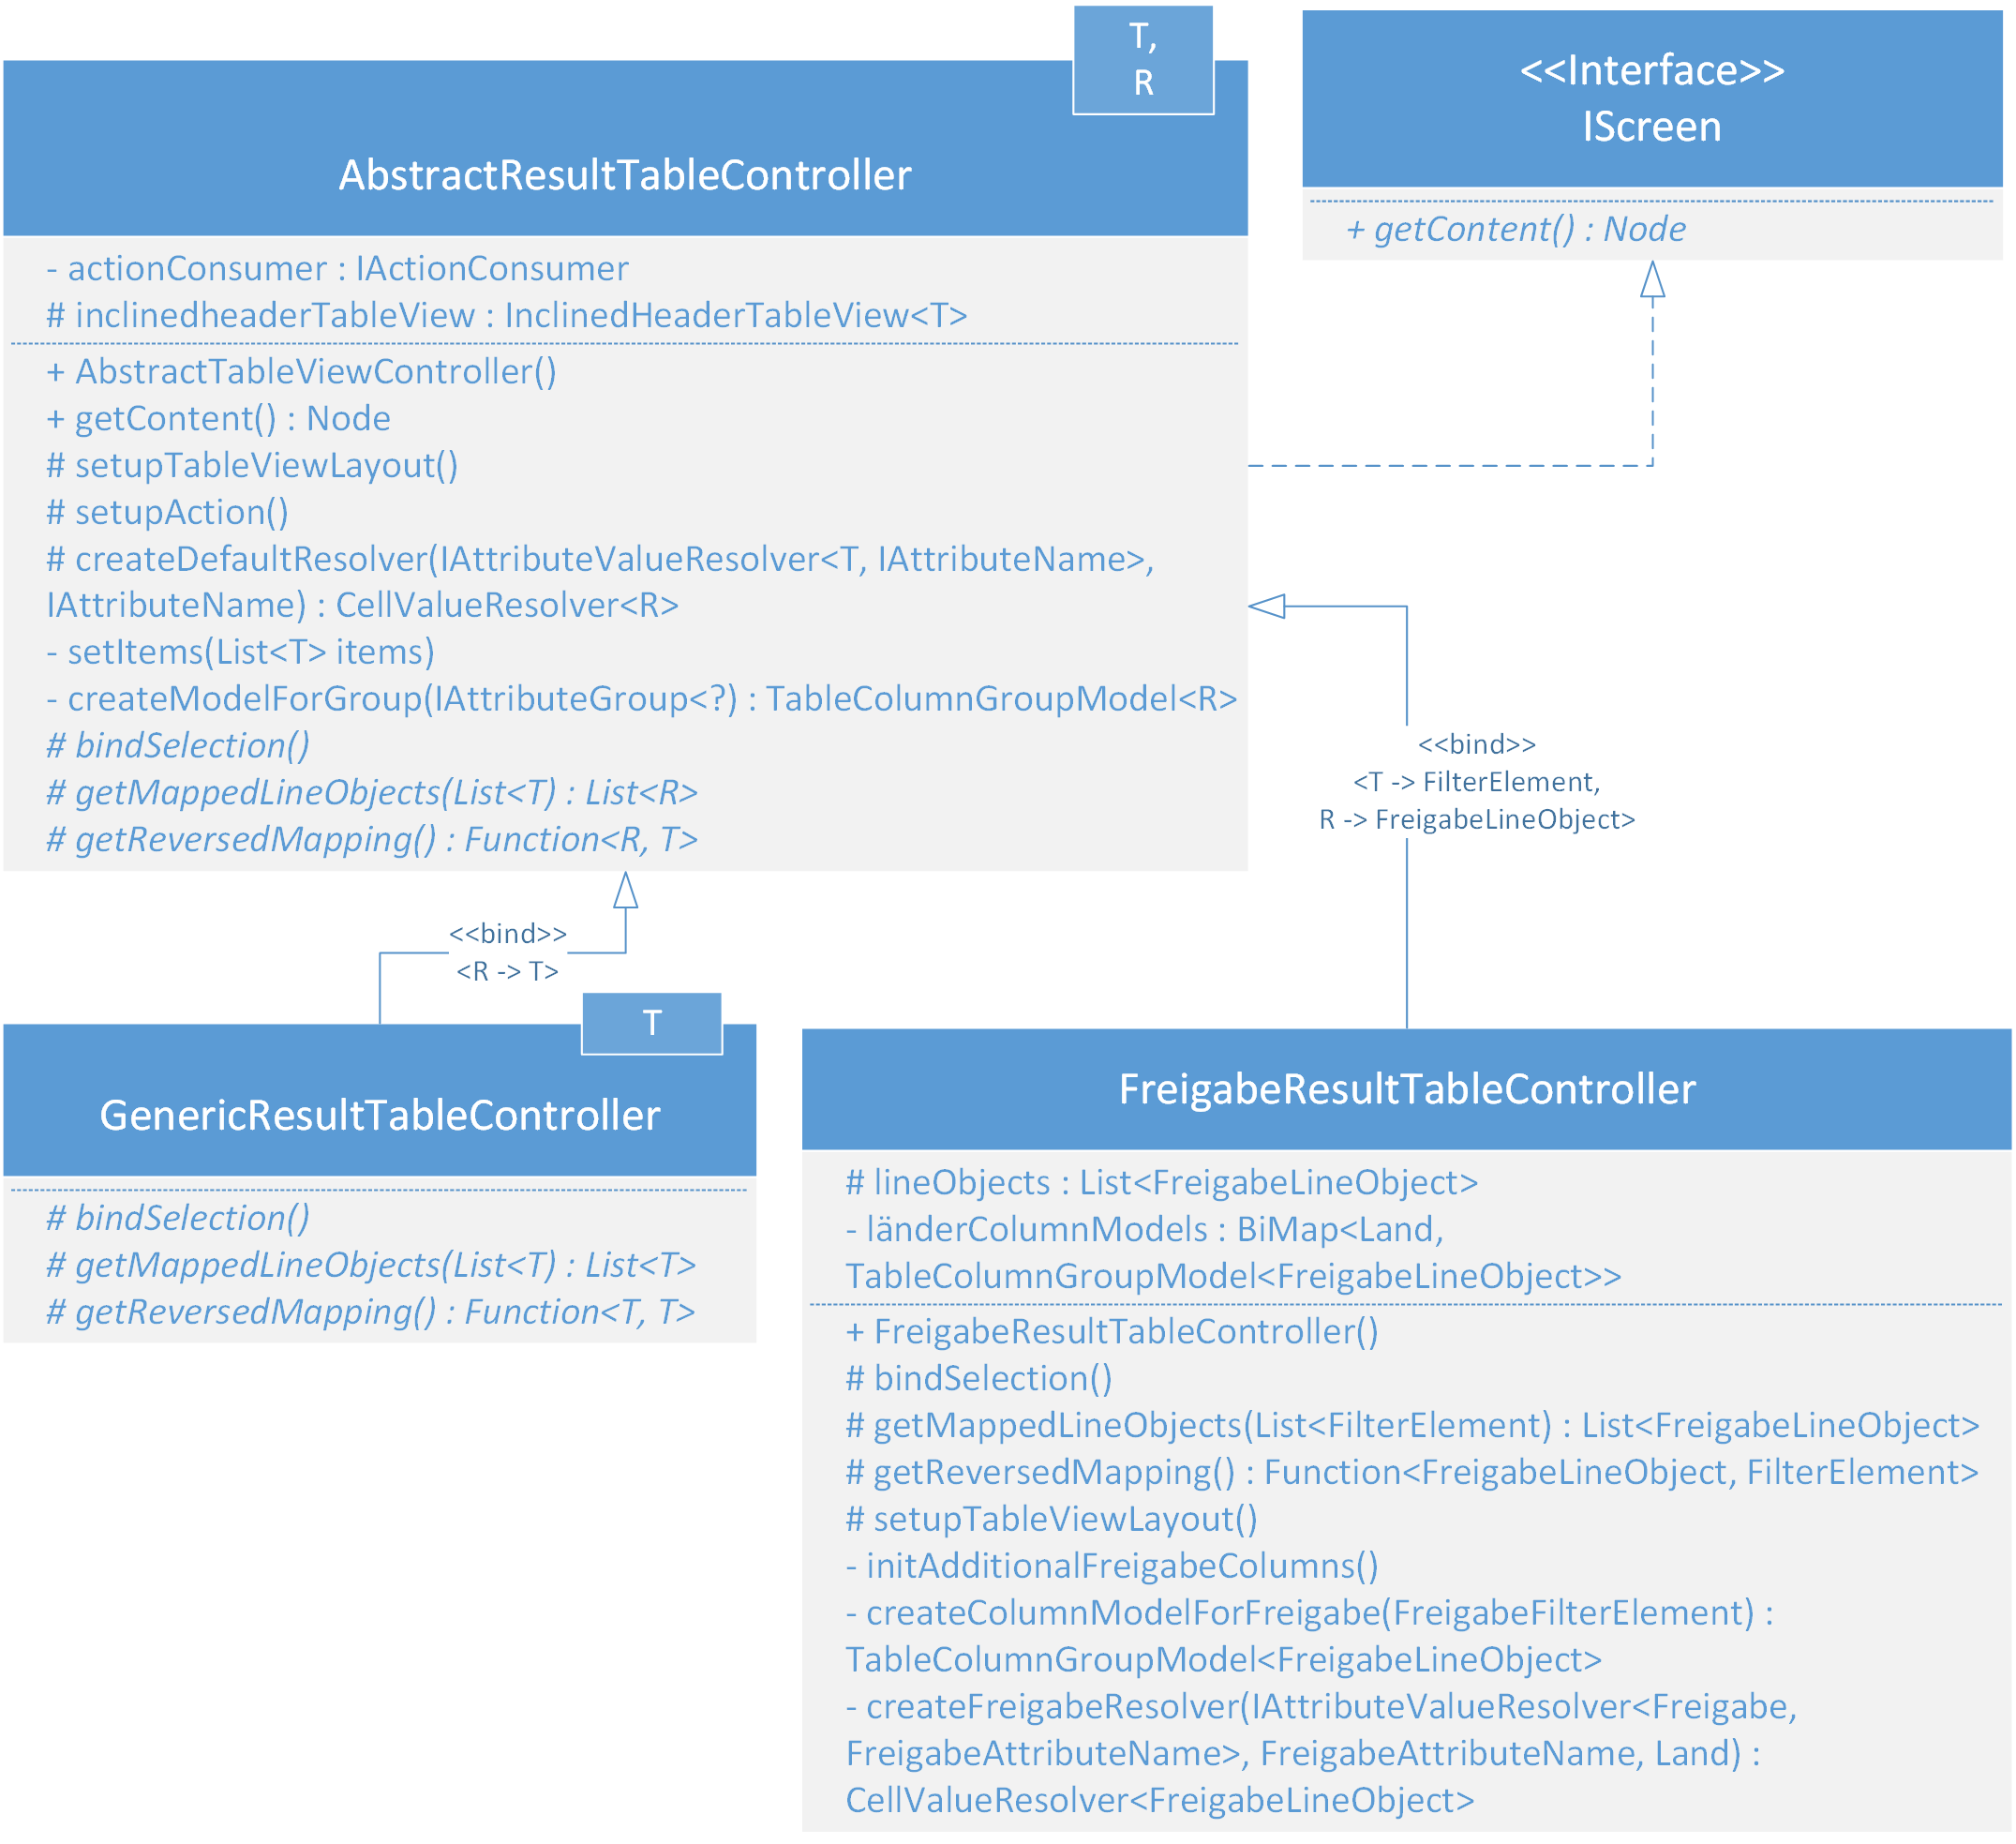
\includegraphics[width=1.0\textwidth]{grafiken/Class_ResultTable.png}
 \caption{Klassendiagramm Ergebnisansicht}
 \label{fig:tabelle4}
\end{figure}

Für die zu überschreibenden abstrakten Klassen ist die Implementierung des GenericResultTableControllers denkbar simpel.


\begin{lstlisting}[
    language=Java,
    caption=GenericResultTableController - Mapping-Methoden,
    label=code10]
	public List<T> getMappedLineObjects(List<T> data) {
		return data;
	}

	public Function<T, T> getReversedMapping() {
		return Function.identity();
	}
\end{lstlisting}

Bei dem FreigabeResultController fällt die Umsetzung etwas komplizierter aus. Bereits beim Konstruktoraufruf werden die Modelobjekte der Ergebnismenge in die Zeilenobjekte "verpackt". Zu diesem Zweck gibt es eine Membervariable vom Typ List<FreigabeLineObject>. Diese Liste wird befüllt, indem für jedes Element aus der Ergebnismenge zunächst ein Zeilenobjekt erstellt wird, das dieses Element enthält. Daraufhin wird mit der List\#contains(Object o)- Methode überprüft, ob dieses Element schon in der Liste vorhanden ist. Dafür wird die \#equals()-Methode der Zeilenobjekte aufgerufen. Da diese überschrieben wurde, liefert sie genau dann true zurück, wenn die ID des zugeordneten Fahrzeuges bei beiden Zeilenobjekten gleich ist. Ist das der Fall, kann das überprüfte FilterElement dem bestehenden hinzugefügt werden, andernfalls wird das erzeugte FreigabeLineObject in die Liste der Zeilenobjekte eingegliedert. Die \#getMappedLineObjects()-Methode kann diese Liste nun sortiert zurückgeben.

Der Vorteil daran, dass die Liste schon zuvor beim Konstruktoraufruf erzeugt wird, und nicht erst bei Bedarf, ist der, dass die Benutzeroberfläche nicht "einfriert". Die Methode \#getMappedLineObjects() wird nach dem Aufbauen der Benutzeroberfläche im GUI-Thread ausgeführt. Wenn die Liste schon vorher erzeugt wurde, fällt an dieser Stelle der Großteil des Rechenaufwandes weg und der Aufbau der Oberfläche erscheint flüssiger.

Während der Konstruktionsphase werden, neben dem Tabellenlayout für die Spalten der Fahrzeugattribute, auch die zusätzlichen Freigabe-Spalten erzeugt, die nach Ländern gruppiert sind und das Start- und Enddatum als konkrete Spalten aufweisen. Auch hier werden wieder die Ergebnisdaten benötigt.

Als erster Schritt wird eine Map erzeugt, die für jedes Land aus der Ergebnismenge ein ColumnGroupModel verwaltet. Als technische Ausprägung dieser Map wird eine HashBiMap aus der Google Guava Library verwendet. Die Besonderheit und der Zweck dieser Datenstruktur werden später erläutert. Durch Java 8– Features kann der grundlegende Code für die Erzeugung der Map relativ gering gehalten werden.

\begin{lstlisting}[
    language=Java,
    caption=Erzeugung der BiMap,
    label=code11]
	countryColumnModels = HashBiMap.create(
			ucContext.getResultData().stream()
			.collect(Collectors.toMap(
					freigabe -> freigabe.getLand(),	// Erzeugung des Keys
					this::createColumnModelForFreigabe, // Erzeugung des Wertes
					(o1, o2) -> o1	// Merge-Function, falls 2 Keys gleich
	 		))
	);
\end{lstlisting}

Die Methode \#createColumnModelForFreigabe() erstellt auf Basis eines beliebigen FilterElements eine TabellenGruppe mit den beiden Spalten für das Start- und Enddatum der Produktionsfreigabe. Dazu gehört ein CellValueResolver, der für eine Zelle dieser Spalte anhand des darunterliegenden Zeilenobjektes den Wert dieser Zelle bestimmen kann. Beim Erstellen des CellValueResolvers wird die Länderinformation aus dem FilterElement übergeben. Anhand der Länder-ID kann dann der richtige Wert für eine Zelle aus dem Zeilenobjekt ermittelt werden. Schlussendlich müssen die Spaltengruppen aus der Map nur noch sortiert werden und der angepassten TableView hinzugefügt werden.

In Abbildung 3.14 wird ersichtlich, dass der FreigabeResultTableController über eine weitere Methode verfügt, die hier von Relevanz ist – die \#bindSelection()-Methode. Diese sorgt dafür, dass das selektierte Modelobjekt, das global (im sogenannten Context) verfügbar ist, aktuell gehalten wird. An diese Selektion ist beispielsweise die Sidebar gebunden, in der es eine Ergebnisvorschau gibt, die das derzeit angewählte Element farblich differenziert darstellt. Um dies in der komplexen Tabelle des 3. Anwendungsfalles zu ermöglichen, wird an die JavaFX-Property der selektierten Zellen ein Listener angehängt. Darin wird die TablePosition der Selektion bestimmt, durch welche die Spalte bestimmt werden kann, in der die Selektion stattgefunden hat. Problematisch ist es jetzt jedoch, das eigentliche Modellobjekt (vom Typ FilterElement) zu identifizieren, da über die Selektion nur das Zeilenobjekt erhalten werden kann. Zur Erinnerung: Um von einem FreigabeLineObject auf ein FilterElement schließen zu können, wird das Länderobjekt benötigt. An dieser Stelle kommt die zuvor erwähnte HashBiMap ins Spiel. Diese hat nämlich die Eigenheit, dass sowohl die Keys als auch die Values eindeutig zu identifizieren sind. Es entsteht also eine eineindeutige Beziehung zwischen den Objekten. Aus diesem Grund lassen sich die eigentlichen Values auch als Keys verwenden. Durch den Aufruf \#inverse() auf der BiMap wird diese invertiert und die vorherigen Keys werden zu Values und umgekehrt. Durch die zuvor ermittelte Spalte kann das dazugehörige Spaltengruppenmodell identifiziert werden und dadurch das zugehörige Land (aus der invertierten BiMap). Mit Hilfe des Landes lässt sich nun auf das Modellobjekt schließen, das daraufhin im Context aktualisiert wird.

Die letzte verbliebene Methode ist \#setupAction(). Der Zweck dieser Methode ist das Ermöglichen von Interaktionen mit der Tabelle. Zum Beispiel kann bei einem Doppelklick eine Detailansicht zu einem selektierten Modellobjekt angezeigt werden.

Zur größeren Übersichtlichkeit bei der Navigation durch die umfangreiche Tabelle, wird neben der Zelle, die derzeit selektiert ist, auch die Spalte in einem helleren Farbton mit eingefärbt. So lässt sich schnell das zu einer Freigabe gehörende Fahrzeug identifizieren. Aufgrund der Tatsache, dass eine JavaFX TableView nur entweder Reihenselektion oder Zellselektion nativ unterstützt, musste eine andere Lösung für das Hervorheben gefunden werden. Diese bestand in dem Setzen einer selbst definierten CSS-Pseudoklasse, die genau dann auf eine Zeile angewandt wird, wenn Zellselektion aktiviert ist und eine Zelle aus der betroffenen Zeile selektiert wurde. Andernfalls würden die Standard-CSS-Definitionen für Tabellenzeilen angewandt werden.
\chapter{Analyse ausgewählter Usability-Probleme}
\section{Situation} \label{sec:analyseSituation}
In einer Liste werden Texte angezeigt, die aus zwei Teilen bestehen. In einem Fall ist der erste Teil ein Schlüssel zur Identifizierung eines Fahrzeuges, der zweite Teil ist der Name des Fahrzeuges. Ein Fahrzeugname kann unter Umständen mehr als einmal auftreten, der Fahrzeugschlüssel hingegen ist eindeutig. Während die Schlüssel sich in der Zeichenanzahl nur um 2-3 Zeichen unterscheiden, können die Fahrzeugnamen ganz unterschiedliche Längen haben. Derzeit werden die beiden Textbausteine schlicht aneinandergereiht. Dies führt bei längeren Listen schnell zu Unübersichtlichkeit. Daher sollte eine sichtbare Trennung zwischen den beiden Elementen erfolgen.

\begin{figure}[H]
 \centering
 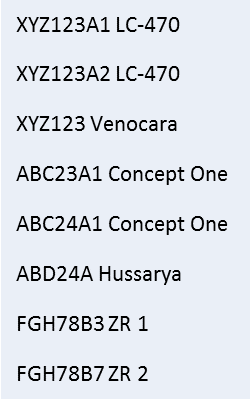
\includegraphics[width=0.3\textwidth]{grafiken/Liste_Beispiel.png}
 \caption{Liste: Ausgangszustand}
 \label{fig:liste1}
\end{figure}

\begin{figure}[H] 
	\centering
	\subfloat[Design 1] {
		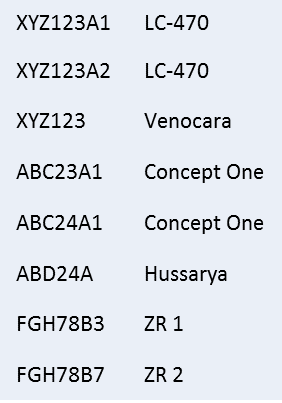
\includegraphics[width=0.3\textwidth]{grafiken/Liste_Design1.png}
	}
	\hspace{1.0em}
	\subfloat[Design 2] {
		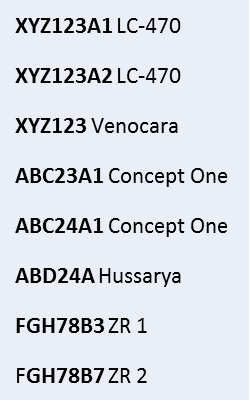
\includegraphics[width=0.265\textwidth]{grafiken/Liste_Design2.png}
	}
	\hspace{1.0em}
	\subfloat[Design 3] {
		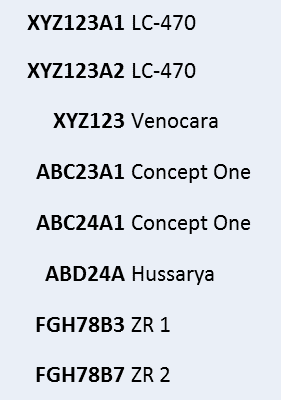
\includegraphics[width=0.3\textwidth]{grafiken/Liste_Design3.png}
	}
	\caption{Design-Vorschläge}
	\label{fig:liste2}
\end{figure}

Alle Design-Vorschläge sind valide Möglichkeiten zur Lösung des Problems, haben jedoch auch ihre Vor- und Nachteile.

Der erste Designvorschlag (Abbildung 4.2) stellt die beiden Teile des Textes sehr gut optisch getrennt dar. Beide Teile sind tabellenartig linksbündig angeordnet. Die ID-Teile aller Texte sind dabei auf einer Höhe, genauso wie die Namensteile. Auf diese Weise entstehen zwei Spalten, in denen die Textbausteine dargestellt werden.

Bei dem zweiten Designvorschlag (Abbildung 4.3) ist der linke Teil des Textes fett gedruckt, der andere Teil in ganz normalem Stil. Die zweite Lösung setzt zwar die Trennung nicht so "sauber" wie Vorschlag 1 um, stellt aber so die Fachlichkeit besser dar. Die Fahrzeug ID und der Fahrzeugname sind eine zusammengehörige Einheit. Nach dem Gestaltgesetz der Nähe (Kapitel 2.5.1) würden bei Designvorschlag 1 die Fahrzeugschlüssel als eine Objektgruppe und die Fahrzeugnamen als eine Objektgruppe gesehen werden. Da dies nicht die Intention der Abbildung ist, eignet sich die zweite Lösung besser für die Lösung des Problems.

Der dritte Vorschlag gruppiert die Elemente der Liste zwar ebenso wie in Abbildung 4.3, ist jedoch eine eher exotische Darstellungsweise. Hier sind die Elemente an einer gedachten senkrechten Linie zwischen den beiden Teilen angeordnet. Durch die unterschiedliche Bündigkeit entsteht der Eindruck der Gruppierung pro Element, ebenso wie in Vorschlag 2. Durch das Fettdrucken der linken Spalte wird diese dazu hervorgehoben. Das Problem dieser Darstellungsweise ist jedoch der Stilbruch zu den anderen Listendesigns, die im gleichen Bereich angezeigt werden können. Die anderen darstellbaren Listen beinhalten größtenteils keine 2-teiligen Texte. Auf diese Standardvariante der Listen könnte das dritte Design nicht angewandt werden. Es würde daher das Gesetz der Ähnlichkeit (Kapitel 2.5.1) verletzt werden und sich so unter Umständen unangenehm auf das Nutzerempfinden auswirken.
\section{Filter-Performance} \label{sec:analyseFilterPerformance}
Die Änderungen, die in Kapitel 3.1 eingeführt wurden, funktionieren zwar aus technischer Sicht, lassen den Filter aber bei bestimmten Operationen langsam arbeiten, was zu unbequemen Verzögerungen führt.

\textbf{Analyse}

Um die Laufzeitprobleme beheben zu können, mussten als erstes die Fehler gefunden werden, die zu besagten Problemen führten. Bei der Analyse wurden die folgenden Problemfaktoren untersucht:

\begin{itemize}
	\item Zeitintensive Anweisung (möglicherweise in Schleifen ausgeführt?)
	\item Mehrfach hinzugefügte JavaFX-Listener an ObservableLists
	\item Schleifen mit hohen Durchlaufzahlen
	\item Konstruktion von vielen, großen Objekten
\end{itemize}

Für die Überprüfung des ersten Faktors mussten alle Anweisungen einzeln angeschaut werden. Wenn ein Funktionsaufruf dabei ist, der viele Berechnungen ausführt, kann die Ausführungszeit des Aufrufes dadurch gemessen werden, dass der Zeitpunkt vor der Ausführung gespeichert wird und nach der Ausführung von der dann aktuellen Zeit abgezogen wird. Benutzt dafür den Aufruf System\#currentTimeMillis() erhält man die Zeitspanne in Millisekunden. Auf diese Weise ließ sich kein performancekritischer Methodenaufruf feststellen. Auch unter Berücksichtigung, dass manche Methoden in Schleifen ausgeführt werden, fand sich keine kritische Stelle.

Die zweite Überprüfung war erfolgreicher. Tatsächlich wurden zwar keine Listener mehrfach an einer ObservableList angehängt, aber pro Werteliste im Filter (in diesem Fall 13) wurden jeweils einige Listener ausgelöst, die diese aktualisieren sollten, wenn sich die ausgewählten Werte geändert haben. Diese Berechnungen erforderten einigen Aufwand und dadurch, dass sie, statt einmal, 13-mal ausgeführt wurden, sorgten sie für eine negative Laufzeitbeeinflussung.

Diese Lösung dieses Problems alleine brachte jedoch nicht den gewünschten Effekt. Eine Methode, die extrem oft ausgeführt wurde und für die meisten Filterberechnungen relevant ist, ist die Methode, die in der Menge der selektierten Werte sucht, ob eine Attribut-Werte-Kombination vorhanden ist.

\begin{lstlisting}[
    language=Java,
    caption=Aufbau - selectedValues,
    label=code12]
	ObservableList<Pair<AbstractFilterAttribute<A>, Object>> selectedValues;
\end{lstlisting}

Als Parameter erhält die Methode ein Attribut und einen Wert, der überprüft werden soll. Die aufgerufene benutzt die \#contains(Object)-Methode der List-Implementierung. Dafür muss für jede Überprüfung ein Objekt vom Typ Pair erzeugt werden, das das Attribut und den zu überprüfenden Wert kapselt. Zudem muss danach (durch die Implementierung von \#contains(Object)) jedes Objekt der Liste durchlaufen werden und per \#equals(Object) verglichen werden. Je größer die Menge der ausgewählten Werte wird, desto öfter muss ein solcher Vergleich ausgeführt werden. Die Laufzeit eines Durchlaufes über diese Datenstruktur $O(n)$. Bei einzelnen Aufrufen würde dies nicht weiter problematisch werden, doch durch den neuartigen Filter wird diese Methode nun weitaus häufiger ausgeführt.

\textbf{Quellcode-Usability}

Die Java 8 -Sprachfeatures sind ein gutes Mittel, vor Allem in Kombination mit JavaFX und der Stream-API, Code prägnant und sehr kurz darzustellen. Doch haben die neuen Features, vornehmlich Lambdas auch die Eigenschaft, Code schnell zu verkomplizieren, wenn sie im Überfluss verwendet werden. Der durch die Definition bestimmte Nachteil eines Lambdas ist, dass nicht sofort erkennbar ist, welches Interface implementiert wird und was die Parameter zu bedeuten haben. Dies lässt nicht nur ungeübte Java 8 –Programmierer an einigen Codestellen verzweifeln. Ein Konstrukt, das im Quellcode in einer noch ausgeprägteren Variante zu finden war, wird folgend umrissen.

\begin{lstlisting}[
    language=Java,
    caption=Code-Qualität - Gegenbeispiel,
    label=code13]
	boolen hasSubLevels = level.getListEntries().stream().filter(
			entry -> entry instanceof ILevel).count() > 0;
	entryList.setCellFactory(list -> new ListCell<IListEntry>() { 		//1
		{ setPrefWidth(0); } 																//2
		@Override
		protected void updateItem(IListEntry item, boolean empty) {
			super.updateItem(item, empty);
			[...]
			FalkoArrow arrow = new FalkoArrow(Direction.LEFT);
			arrow.setOpacity(item instanceof ILevel ? 1.0 : 0.0); 			//3
			[...]
			HBox hbox = new HBox(5.0);
			if (hasSubLevels) {
				hbox.getChildren().add(arrow);
			}
			[...]
			setOnMouseClicked((v) -> doCallback(item)); 						//4
			setCursor(empty ? Cursor.DEFAULT : Cursor.HAND);
		}
	});
\end{lstlisting}

Der Code ist zwar sehr knapp aber führt selbst mit Syntax-Coloring schnell zur Unübersichtlichkeit. Dieser Effekt wird dadurch verstärkt, dass das selten verwendete Konstrukt des Instanz-Initializers (2), kombiniert mit einer Anonymen Inneren Klasse als Rückgabewert eines Lambdas eingesetzt wird (1). In dieser Klasse werden zusätzlich ternäre Ausdrücke als Alternative zu If-Klauseln (3) und weitere Lambdas (4) benutzt. Zudem hat die Anonyme Innere Klasse Referenzen in den umschließenden Block (Variable hasSubLevels).

Ein weiteres Beispiel hängt mit der Verwendung des Double-Colon-Operators zusammen:

\begin{lstlisting}[
    language=Java,
    caption=Code-Qualität - Gegenbeispiel 2,
    label=code14]
	protected StringProperty specialTextProperty = new SimpleStringProperty("[all values]");
	protected final IListEntry specialEntry = specialTextProperty::get;
\end{lstlisting}

Auch über diesen sehr kurzen Code-Ausschnitt kann sich schnell der Kopf zerbrochen werden. Ein JavaFX StringProperty hat nur die Funktion, einen String-Wert zu kapseln und den Zugriff darauf zu erlauben - über die Funktion \#get() und \#set(String). Warum ist der obenstehende Code nicht fehlerhaft? Liefert \#get() in diesem Falle doch keinen String zurück?
Es sieht in der Tat für ungeübte Java 8 -Entwickler so aus, als würde der Variable "specialEntry" ein String zugewiesen werden. Doch hier handelt es sich um die Kurzschreibweise eines Lambda-Ausdruckes. Die betroffene Zeile würde wie folgt in einen "echten" Lambda übersetzt werden:

\begin{lstlisting}[
    language=Java,
    caption=Code-Qualität - Verbesserung,
    label=code15]
	protected final IListEntry specialEntry = () -> specialTextProperty.get();
\end{lstlisting}

Um den Sinn genauer verstehen zu können, muss das Interface IListEntry genauer angeschaut werden. Hier befinden sich zwei Methoden. Eine Default-Implementierung für die Methode \#getText() und die abstrakte Methode \#getValue(), die die String-Repräsentation von \#getValue() zurückliefert. Es muss also die Methode \#getValue() des funktionalen Interfaces implementiert werden, damit eine vollständige Klasse entsteht. Genau das machen beide obige Code-Ausschnitte. Dennoch ist die Schreibweise zunächst unverständlich.

Dies sind nur zwei Beispiele für schwierig lesbaren Code, im Laufe eines Java 8 -Projektes können viele solcher und ähnlicher Probleme auftreten.
\chapter{Implementierung der Usability-Verbesserungen}
\section{Präsentation von 2-teiligen Texten in ListCells} \label{sec:verbListCell}
Die Umsetzung des zweiten Designvorschlages ist nicht so einfach möglich, wie die Grafik zunächst vermuten lässt. Es ist standardmäßig nicht möglich den Text, der in dem Textbereich einer ListCell eingefügt werden soll zu teilen und zwei verschiedene Styles darauf anzuwenden.

Wenn man nicht die ListCell-Klasse erweitern und stark verändern möchte, bleibt nur die Möglichkeit, über die Graphic, die gesetzt werden kann, einen Text einzufügen. Die Graphic entspricht hier nicht einer Grafik im allgemein gebräuchlichen Sinne, sondern einem JavaFX Node, der eine beliebige Ausprägung haben kann. So könnten in der Theorie auch sehr komplexe Elemente als Listenelemente dargestellt werden.

Der Text, der in den Listenzellen angezeigt werden soll, erhält die Klasse aus dem DataProvider. Dieser fügt die Teile der Texte bisher zusammen und liefert sie als einen einzelnen String zurück. Bei der Präsentation werden jedoch Teilstrings benötigt. Nun könnte der Text geparst werden und daraufhin wieder aufgespalten, allerdings wäre dieses Vorgehen nicht sinnvoll, da die gleiche Listenzelle auch für Texte funktionieren soll, die nicht aufgeteilt sind. Möglicherweise würde der Text in dem Fall sogar fälschlicherweise fettgedruckt werden. Aus diesem Grund müssen die Texte von vorneherein als Mehrteiliger Text aus dem DataProvider geliefert werden. Die naheliegendste Lösung ist es, ein Array zu benutzen, das die Textteile speichert. Aufgrund der Tatsache, dass die Rückgabewerte aus dem DataProvider auch an anderen Stellen verwendet werden, muss sich das zurückgegebene Objekt nach außen hin wie ein String verhalten. Dies kann dadurch erreicht werden, dass das Array in ein neues Objekt verpackt wird, welches die \#toString()-, \#hashCode()- und \#equals(Object)- Methoden überschreibt und die einzelnen Textteile zuvor zu einem String zusammenfügt.

Die Listenzelle muss jetzt nur noch überprüfen, ob es sich bei dem zurückgelieferten Wert um ein Objekt der Klasse MultiPartString handelt und kann daraufhin den ersten Teil des Textes anders darstellen.

Für das korrekte Layout wird ein sogenannter TextFlow verwendet, der die Abstände zwischen den Textpassagen so einstellt, dass die Teile wie ein einziger Fließtext wirken.

\section{Filter-Performance} \label{sec:verbFilterPerformance}
\textbf{Behebung: Listenaktualisierung}

Um die Menge an gleichzeitigen Listenaktualisierungen zu reduzieren muss zunächst definiert werden, welche Listen zu welchem Zeitpunkt aktualisiert werden müssen. Das ist zunächst die Liste, die zum aktuellen Zeitpunkt angezeigt wird - die anderen Listen sind dann zwar zeitweise veraltet, dies fällt dem Nutzer jedoch nicht auf, da er die Listen nicht sehen kann. Allerdings muss dann jedes Mal, wenn eine andere Werteliste angezeigt werden soll, diese Liste ebenfalls aktualisiert werden, bevor sie dem Nutzer angezeigt wird.

Das ganze kann nur ermöglicht werden, wenn eine Koppelung mit der Benutzeroberfläche stattfindet. Jedes Mal, wenn der Nutzer ein anderes Attribut auswählt, um die dazu passende Werteliste zu erhalten, wird eine Methode im Filter ausgeführt, die als Parameter das jetzt aktive Attribut erhält. Die dazu gehörige Werteliste wird dann einmal erneuert und nur diese durch den Listener aktuell gehalten.

\textbf{Behebung: Zugriff auf selektierte Werte langsam}

Das Problem der Menge der selektierten Werte musste auf Ebene der Datenstruktur angegangen werden. Je nachdem, wie viele Werte bereits selektiert waren, konnten sich die Laufzeiten für die Suche in dieser Struktur auf insgesamt bis zu mehrere Sekunden verlangsamen (kumulierter Gesamtwert aller Ausführungen, die bei einer Neuselektion eines Attributwertes nötig sind).

Für den schnelleren Zugriff wurde eine weitere Datenstruktur eingeführt, die eine andere Repräsentation der selektierten Werte darstellt. Durch eine HashBasedTable, einer Struktur aus der Google Guava Bibliothek, war es möglich, die Laufzeitkomplexität für einen Zugriff auf die selektierten Werte von $O(n)$ auf $O(1)$ zu verkürzen. Die Struktur ähnelt einer HashMap, arbeitet jedoch auf zwei Dimensionen und bietet die Möglichkeit, 2 Keys zu verwenden, um einen Wert zu erhalten. Da die Zeitdauer zum Auffinden eines solchen Keys in beiden Dimensionen der HashBasedTable konstant ist, ist ein sehr schneller Zugriff auf Elemente möglich.

\begin{lstlisting}[
    language=Java,
    caption=Datenstruktur - FastSelectedValues,
    label=code16]
	private HashBasedTable<AbstractFilterAttribute<A>, Object, Object> fastSelectedValues;
\end{lstlisting}

In obigem Code-Beispiel wird die Zusammensetzung der neuen Datenstruktur gezeigt. Der erste generische Parameter steht für das Attribut, der zweite für den gesuchten Attributwert. Der dritte Parameter wird nicht verwendet und enthält nur der Boolean-Wert true, damit ein Objekt für das Key-Paar vorhanden ist. Die Existenz eines Key-Paares kann dann mit \#contains(Object, Object) überprüft werden. Die Laufzeit verringert sich dadurch von anfänglich mehreren Sekunden auf wenige Millisekunden. Um unnötigen Rechenaufwand zu vermeiden, wird die Struktur nur einmal aktualisiert, sobald sich die selektierten Werte verändert haben. Ein weiterer Vorteil ist, dass die Erzeugung von vielen Objekten des Typs Pair wegfällt.

\textbf{Quellcode-Usability}

Um das erste in Kapitel 4.3 dargestellte Usability-Problem zu lösen, kann zum Beispiel die Anonyme Innere Klasse extrahiert werden und als eigenständige Klasse in einer eigenen Datei implementiert werden. Dadurch fiele außerdem der Instance Initializer weg, dessen Code stattdessen im Konstruktor ausgeführt werden kann. Referenzen in den übergeordneten Scope werden dem Konstruktoraufruf als Parameter übergeben.

Das zweite Problem erübrigt sich, wenn auf den Lambda-Ausdruck verzichtet und stattdessen eine Anonyme Innere Klasse implementiert werden würde.

Das Problem der Quellcode-Usability ist jedoch ein grundlegenderes. Zur Lösung müssen Richtlinien festgelegt werden, wann, in welchem Maße und in welchen Kombinationen Lambdas und andere Sprachfeatures verwendet werden dürfen.

Einige mögliche Richtlinien sind zum Beispiel folgende:

\begin{itemize}
	\item Keine Anonymen Inneren Klassen innerhalb von Lambdaausdrücken verwenden
	\item Lambdas in maximal 2 bis 3 Ebenen schachteln
	\item Bei Schachtelung von Lambdas stets durch Einrückungen kennzeichnen
	\item DoubleColon-Operator nur in selbsterklärenden Fällen
\end{itemize}

Die Liste ist weit entfernt davon, komplett zu sein, aber vermittelt dennoch einen kurzen Eindruck, wie Lese- und Verständnisschwierigkeiten im Quellcode vermieden werden können.
\chapter{Ausblick und Fazit}
Durch die Entwicklung ist das Projekt einen großen Schritt in Richtung Release vorangekommen. Die Weiterentwicklung der bestehenden Funktionen verbessert nicht nur die Gebrauchstauglichkeit der Anwendung, sondern eröffnet dem Endanwender auch ganz neue Möglichkeiten, die Software zu verwenden.
Die Intention hinter dem Produkt ist durch die Entwicklung weiter verfolgt worden und so wird dem Nutzer eine zwar eingeschränkte, aber weitaus übersichtlichere Möglichkeit dargeboten, Daten aus dem \gls{falko}-System zu betrachten und auszuwerten.
Dennoch sind noch einige Arbeiten vorzunehmen, bevor von einem vollständigen Funktionsumfang gesprochen werden kann und gerade im Kernaspekt der Anwendung, der \gls{gebrauchstauglichkeit}, besteht noch viel Evaluations- und Optimierungsbedarf.

\bibliography{biblio/biblio}
\listoffigures
\listoftables

\printglossaries

\appendix
ethjnjdgjsfgjsrmk

\end{document}